\documentclass[12pt,a4paper]{report}

\usepackage[pdftex]{graphicx}
\DeclareGraphicsExtensions{.pdf,.jpeg,.png,.jpg}
\usepackage{amsthm,amssymb} % for mathematical formulas
\usepackage{rotating} %used to have landskape figures
\usepackage{graphicx}
\usepackage{enumerate}
\usepackage{epsfig}
\usepackage{algorithms}
\usepackage{makeidx}



   % to have links to figures and citations in PDF version.
\usepackage{hyperref}

\usepackage{setspace}
\renewcommand{\baselinestretch}{1.5}
%\renewcommand{\bibname}{References}

\pagestyle{headings}  % to get running heads
\makeindex


%------------------------- Document settings ------------------------
\topmargin   0mm
\hoffset     0mm
\voffset     0mm
\textwidth   150mm
\textheight  220mm
%------------------------- Definitions ------------------------------

\renewcommand{\theenumi}{\alph{enumi}} % to get alphabets in enumerated lists
\renewcommand{\theenumii}{\arabic{enumii}} % to get numbers in level-2 enumerated lists
\renewcommand{\thetable}{\Roman{table}} % to get table numbers in capital roman
\renewcommand{\chaptername}{Chapter}
\renewcommand{\textwidth}{6in}
\newcommand{\pic}[2]{\setlength{\epsfysize}{#1} \epsffile{#2}}
%------------------------- document ---------------------------------

\begin{document}
% --------- Title and abstract etc the front matter -----------
\pagenumbering{roman}
% TITLE PAGE

\thispagestyle{empty}
\begin{center}
%\vspace{1cm}
{\LARGE \bf DEVELOPMENT OF GNU/LINUX DISTRIBUTIONS }\vspace{.01in}\\
\end{center}
\begin{center}
{\bf B. Tech Computer Semester - VIII}\\
Prepared At
\end{center}
\begin{figure}[h]
\begin{center}
  % Requires \usepackage{graphicx}
  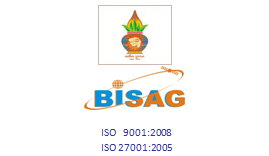
\includegraphics [scale=0.47] {Bisag.png}\\
\end{center}
\end{figure}

\begin{center}
\bf{Bhaskaracharya Institute for Space Applications \& Geo-informatics}\\
\bf{Govt.of Gujarat,Science \& Technology, Gandhinagar}\\

\end{center}
\begin{center}
Prepared By\\
\begin{tabular}{ l p{1 cm} l }
{\large \bf Arpan Chavda} & & {\large \bf Hitesh Piprotar} \\
{\bf 09BCE006} & & {\bf 09BCE054}
\end{tabular}
\\
\vspace{0.35cm}
\begin{tabular}{ l p{1 cm} l }
{\bf Internal Guide,} &  & {\bf External Guide,}\\
{\large \bf Dr. Sanjay Garg} &  & {\large \bf Mr. Miren Karamta }\\
{\bf HOD,} &  & {\bf Project Scientist,}\\
{\bf Dept. of Computer Science \& Engg., } & & {\bf BISAG,}\\
{\bf Institute of Technology,} & & {\bf Gandhinagar}\\
{\bf Nirma University, Ahmedabad} & & \\
\end{tabular}
Submitted to
\end{center}
\begin{figure}[h]
\begin{center}
  % Requires \usepackage{graphicx}
  
\includegraphics [scale = 0.4] {NirmaLogo.png}
\end{center}
\end{figure}
%\pic{60pt}{NirmaLogo.png}\\ ~\\
\begin{center}
{\bf DEPARTMENT OF COMPUTER SCIENCE AND ENGINEERING}\\
{\bf NIRMA UNIVERSITY, AHMEDABAD-382481}\\
{\bf MAY 2013}
\end{center}

% -------------------------------------------------------------------------
\newpage
\thispagestyle{empty}
\begin{center}
%\vspace{1cm}
{\LARGE \bf DEVELOPMENT OF GNU/LINUX DISTRIBUTION}\\
{\large \bf Major Project}\\
Prepared at\\
\begin{figure}[h]
\begin{center}
  % Requires \usepackage{graphicx}
  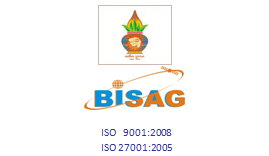
\includegraphics [scale=0.45] {Bisag.png}\\
  \end{center}
\end{figure}
\bf{Bhaskaracharya Institute for Space Applications \& Geo-informatics}\\
\bf{Govt.of Gujarat,Science \& Technology, Gandhinagar}\\
Submitted in partial fulfillment of the requirements for the degree of \\
\textbf{Bachelor of Technology in (Computer Engineering)}\\
Prepared By\\
\begin{tabular}{ l p{1 cm} l }
{\large \bf Arpan Chavda} & & {\large \bf Hitesh Piprotar} \\
{\bf 09BCE006} & & {\bf 09BCE054}
\end{tabular}

\vspace{0.6cm}
\begin{tabular}{ l p{1 cm} l }
{\bf Internal Guide,} &  & {\bf External Guide,}\\
{\large \bf Dr. Sanjay Garg} &  & {\large \bf Mr. Miren Karamta }\\
{\bf HOD,} &  & {\bf Project Scientist,}\\
{\bf Dept. of Computer Science \& Engg., } & & {\bf BISAG,}\\
{\bf Institute of Technology,} & & {\bf Gandhinagar}\\
{\bf Nirma University, Ahmedabad} & & \\
\end{tabular}
\end{center}
\begin{figure}[h]
\begin{center}
  % Requires \usepackage{graphicx}
  
\includegraphics [scale=0.4] {NirmaLogo.pdf}
  \end{center}
\end{figure}
\begin{center}
%\pic{60pt}{NirmaLogo.png}\\ ~\\
{\bf DEPARTMENT OF COMPUTER SCIENCE AND ENGINEERING}\\
{\bf NIRMA UNIVERSITY, AHMEDABAD-382481}\\
\end{center}

% -------------------------------------------------------------------------
    \newpage
    \begin{figure}[h]
    \begin{center}
      % Requires \usepackage{graphicx}
      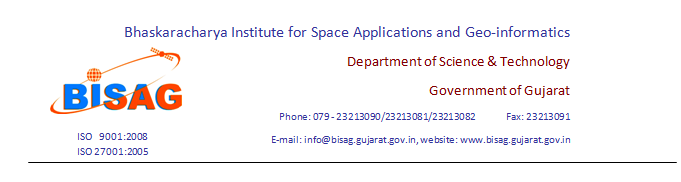
\includegraphics {BisagLogo.png}
    \end{center}
    \end{figure}

\addcontentsline{toc}{chapter}{BISAG Certificate}\label{BISAG Certificate}
\index{BISAG Certificate}
\begin{center}
{\Large \bf BISAG Certificate}\\
\end{center}
\vspace{10pt}
\noindent
This is to certify that the project report compiled by {\bf Mr Arpan Chavda(09BCE006)} and {\bf Mr Hitesh Piprotar(09BCE054)} students of 8th Semester B.Tech from Department Of Computer Science, Institute of Technology, Nirma University have completed their final semester project satisfactorily. To the best of our knowledge this is an original and bonafide work done by them. They have worked on “Development of GNU/Linux Distributions��, starting from January 7th, 2012 to April 24th, 2013.\\
During their tenure at this Institute, they were found to be sincere and meticulous in their work. We appreciate their enthusiasm \& dedication towards the work assigned to them.We wish them every success.
\vspace{3cm}


\noindent
\begin{tabular}{ l l l }
{\bf Mr. Miren Karamta}  & \hspace{3cm} & {\bf T. P. Singh}\\
Project Scientist, &  & Director,\\
BISAG, Gandhinagar & & BISAG, Gandhinagar\\

\end{tabular}
\vspace{2cm}
\noindent

%---------------------------------
% Certificate
%---------------------------------
\newpage
\addcontentsline{toc}{chapter}{Nirma Certificate}\label{Nirma Certificate}
\index{Nirma Certificate}
\begin{center}
{\Large \bf Nirma Certificate}\\
\end{center}
\vspace{10pt}

\noindent This is to certify that the Major Project entitled {\bf "Development of GNU/Linux Distributions"} submitted by {\bf Arpan Chavda (09BCE006)} and {\bf Hitesh Piprotar (09BCE054)}, towards the partial fulfillment of the requirements for the degree of Bachelor of Technology in Computer Engineering of Nirma University, Ahmedabad is the record of work carried out by them under my supervision and guidance. In my opinion, the submitted work has reached a level required for being accepted for examination. The results embodied in this Project work, to
the best of my knowledge, haven't been submitted to any other university or institution for award of any degree or diploma.
\vspace{3cm}

\noindent
\begin{tabular}{ l l l }

{\bf Dr. Sanjay Garg}\\
Head Of Department,\\
Dept. of Computer Science \& Engg.,\\
Institute of Technology,\\
Nirma University, Ahmedabad\\

\end{tabular}
\vspace{2cm}
\noindent

\newpage
\addcontentsline{toc}{chapter}{About the company}\label{About the company}
\index{About the company}
\begin{center}
{\Large \bf About the company}\\
\end{center}
{\bf Introduction of the company}\\
\begin{figure}[h]
\begin{center}
  % Requires \usepackage{graphicx}
  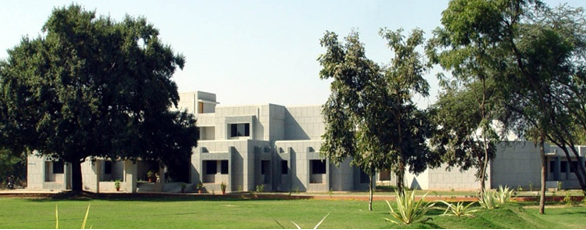
\includegraphics {Campus.png}\\
  \caption[BISAG]{BISAG}
\end{center}
\end{figure}

The applications of space technologies and geo-informatics contribute significantly towards socio-economic development of the society. Recognizing the importance and need of Space technology and geo-informatics for developmental planning purposes, the Government of Gujarat established the Bhaskaracharya Institute for Space Applications and Geo-informatics (BISAG) in the year 1997, as the State nodal agency to utilize space technology and geo-informatics for various developmental activities of the State.

Since its foundation, the Institute has experienced extensive growth in the spheres of space technology and geo-informatics. The objective with which BISAG was established is manifested in the extent of services its renders to almost all departments of the State.  Year after year the institute has been endeavoring to increase its outreach to disseminate the use of geo-informatics up to grassroots level. In this span of eleven years, BISAG has assumed multi-dimensional roles and achieved several milestones to become an integral part of the development process of the Gujarat State.
{\bf Profile}\\
BISAG’s has strengthened its role as a facility provider, a technology developer and as a facilitator for transferring technology to the grass root level.
\begin{figure}[h]
\begin{center}
  % Requires \usepackage{graphicx}
  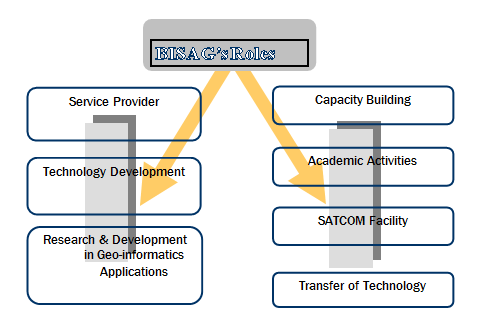
\includegraphics {BisagProfile1.png}\\
  \caption[BISAG's Role]{BISAG's Role}
\end{center}
\end{figure}
Further reinforcing its functions, BISAG has achieved ISO 9001:2008 and ISO 27001:2005 certifications for quality management and security management services respectively. This has led to an organized and systematic development of its services and outputs.\\
{\bf Activities Of BISAG}\\
BISAG’s activities are multi-fold and have expanded in a big way and focused on the following:\\

\begin{itemize}
\item {\bf Satellite Communication :} Promoting and facilitating the use of satellite broadcasting networks for distant interactive training, education and extensions

\item {\bf Remote Sensing :} Inventory mapping, developmental planning and monitoring of natural and man-made resources

\item {\bf Geo-informatics System :} Conceptualizing, creating and organizing multi-purpose common geo-spatial database for sectoral and thematic applications for various users

\item {\bf Photogrammetry :} Creation of Digital Elevation Model, Terrain characteristics, Resource planning,etc.

\item {\bf Global Navigation Satellite System :} Location based services, geo-referencing, engineering applications and research

\item {\bf Software Development :} For providing low-cost Decision Support Systems, desktop as well as web-based geo-informatics applications to users for wider usage.

\item {\bf Disaster Management :} For preparing geo-spatial information to provide necessary inputs to the Government to assess and mitigate extent of damage in the event of a disaster

\item {\bf Education, Research and Training :} For providing education, research and training facilities to promote number of end users through the Academy for Geo-informatics.

\item {\bf Value Added Services :}For providing services which can be customized as per the needs of the users.

\item {\bf Technology Transfer :} Transferring technology to a large number of end users.
\end{itemize}
{\bf Units of BISAG}\\
BISAG initially set up to carry out Space Technology applications, has evolved into an Academic Institute, a Centre for Research and Technology Innovations, a Facility Provider, a Technology Developer and a Facilitator for transferring technology to the grass root level. BISAG is the first such State Centre having such multifarious activities with ISO certification. BISAG has gradually progressed over the years and has grown into several units. Each unit focuses on specific functions and objectives to ensure efficiency in over all activities of the institute.

\begin{itemize}
\item {\bf Gujarat Satellite Communication Network (GUJSAT):} SATCOM facilitates the promotion and facilitation of the use of broadcast and teleconferencing networks for distant interactive training, education and extension.
\item {\bf Centre for Geo-Informatics Applications:} The Centre for Geo-informatics provides services for the developmental and planning activities pertaining to Agriculture, Land and Water Resources Management, Wasteland/ Watershed development, Forestry, Disaster Management, Infrastructure etc.
\item {\bf Software Development:} For wider usage of geo-spatial applications, customised software are developed by the Software Development Team. The institute has provided many indigenous software solutions in the field of Geographic Information Systems, Decision Support Systems and Image Processing.
\item {\bf Academy of Geo-informatics:}  The Academy for Geo-informatics carries out Education, Research and Training activities.
\item {\bf Disaster Management Information cell:} BISAG works closely with the Gujarat State Disaster Management Authority (GSDMA), for assessment of existing situation through integrated analysis and for planning appropriate preventive and preparatory measures, providing necessary support through data generation and analysis.
\end{itemize}

\begin{figure}[h]
\begin{center}
  % Requires \usepackage{graphicx}
  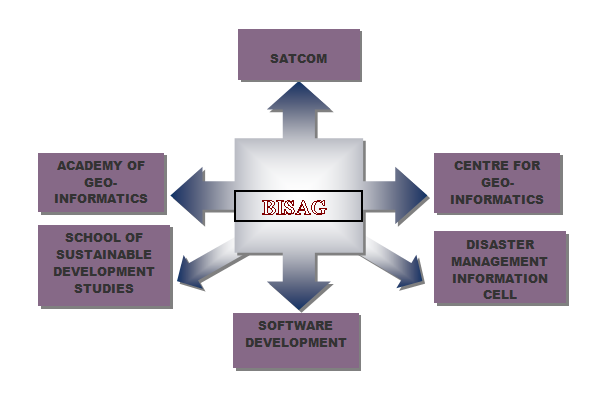
\includegraphics {BisagProfile2.png}\\
  \caption[Units of BISAG]{Units of BISAG}
\end{center}
\end{figure}
\noindent
{\bf Infrastructure Developement}\\
The growth and progress of any institute is gauged by the infrastructure it develops and possesses. BISAG has a sound infrastructure setup that has developed in tandem with the growth of the institute. Having started with one building, there are now dedicated facilities for different units.
The laboratories are equipped with state-of the art technology with latest Hardware and Software required for executing its activities. BISAG also has a rich satellite data archive, which includes Satellite data of different spatial, spectral and temporal resolutions.\\
{\bf Collaborations of BISAG...Creating A Sense Of Ownership}\\
BISAG works with almost all Government Departments and Organizations. Each of these Departments/Organization contributes in preparation of the respective projects. With strong Government support and proactive efforts on part of the staff of BISAG,
\begin{figure}[h]
\begin{center}
  % Requires \usepackage{graphicx}
  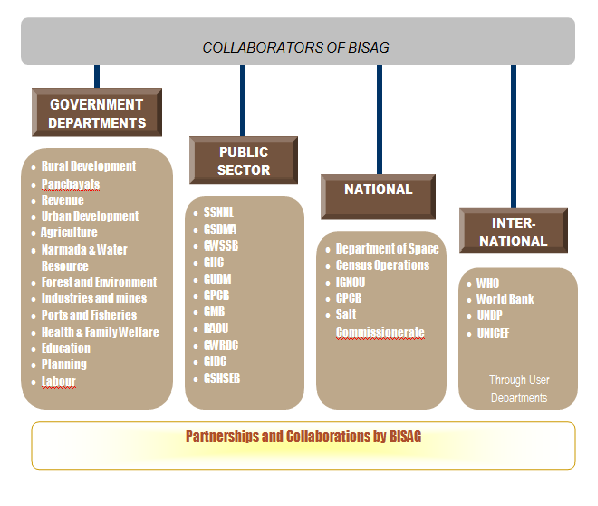
\includegraphics {BisagProfile3.png}\\
  \caption[Partnerships and Collaborations]{Partnerships and Collaborations by BISAG}
\end{center}
\end{figure}
the list of Collaborators is expanding and increasing.\\
{\bf Institutional Strengthening}
BISAG has achieved institutional strengthening through:
\begin{itemize}

\item {\bf Reinforcement of Decision Support Systems}\\
Developing customized solutions as per user requirements through partnerships and collaborations, which are affordable and easy to use. Areas of natural and manmade resources, socio-economic parameters, are being effectively addressed with the help of Geo-informatics.

\item {\bf Establishing Linkage between Government and People through GUJSAT}\\
GUJSAT facility is being constantly employed for the promotion and facilitation of the use of teleconferencing networks for distant interactive training, education and extension. Experts, leaders, specialists and professionals can conduct their programs from a central location reaching out to remote areas through two-way audio-video channel making them interactive and meaningful.

\item {\bf Developing Innovative Education Programmes}\\
Innovative educational programmes are conducted regularly through GUJSAT, allowing people residing in remote areas to have an access to good quality educational and awareness programmes.

\item {\bf Solving real life problems through Human Resource Development}\\
The institute has a young multi-disciplinary team of professionals and a continuing induction programme. Multi-nationals and IT agencies pick up the trained staff that in turn is replaced by new people. This results in availability of more and more trained manpower in the realm of space applications. Every year BISAG provides training to about 300 students in the field of Geo-informatics.


\item {\bf Creation of the multipurpose sectoral comprehensive databases for the entire state of Gujarat}\\
The institute has made efforts towards conceptualization, creation and organization of multi-purpose common digital database for sectoral / integrated decision support systems. This has provided impetus to planning and developmental activities at grass root level as well as monitoring and management potential in various disciplines like water resources, land resources, disaster management, infrastructure, urban management.
\end{itemize}
\newpage
{\bf Communication}\\
The project was undertaken at BISAG, Gandhinagar and BISAG can be contacted at the following:-\\
\vspace{0.14cm}
Near Ch-0 Circle,\\
Indulal Yagnik Marg,\\
Gandhinagar-Ahmedabad highway,\\
Gandhinagar-382007\\
Gujarat,India\\
\vspace{0.14cm}
Phone No:- +91 79 23213081/82/90\\


\newpage
\begin{center}
{\Large \bf Candidate’s Declaration}\\
\end{center}
We declare that final semester report entitled {\bf “DEVELOPMENT OF GNU/LINUX
DISTRIBUTIONS”} is our own work conducted under the supervision of the external guide {\bf Mr. Miren Karamta} from BISAG (Bhaskaracharya Institute for Space Applications \& Geo-informatics).We further declare that to the best of my knowledge the report for B.Tech Computer Science final semester does not contain part of the work which has been submitted for the award of Bachelor Degree either in this or any other university without proper citation.\\
\vspace{1cm}
  \\
Candidate 1’s Signature\\
Arpan Chavda\\
Student ID: 09BCE006\\
\vspace{1cm}
  \\
Candidate 2’s Signature\\
Hitesh Piprotar\\
Student ID: 09BCE054\\
\vspace{1cm}
\\
Submitted To:\\
Department Of Computer Science,\\
Institute of Technology,\\
Nirma University,\\
Ahmedabad.\\

\newpage
\index{Acknowledgements}
\addcontentsline{toc}{chapter}{Acknowledgements}
\begin{center}
{\Large \bf Acknowledgements}\\
\end{center}
\vspace{10pt}
\noindent
Gratitude is a feeling which is more eloquent than words, more tranquil than silence”.

We are grateful to {\bf T.P.Singh}, Director (BISAG) for giving us this opportunity to work the guidance of renowned people of the field of GIS also providing us with the required resources in the company.
We would like to express our endless thanks to our external guide {\bf Mr. Miren Karamta}, Project Scientist at Bhaskaracharya Institute of Space Application and Geo-informatics for their sincere and dedicated guidance throughout the project development.
Also our hearty gratitude to our Head of Department and internal guide, {\bf Dr. Sanjay Garg}  for giving us encouragement and technical support on the project.

The blessings of God and our family members made the way for completion of the major project. We are very much grateful to them.

We are immensely thankful to our friends, who always stood beside and motivated me throughout this course.


\begin{flushleft}
\textbf{ Arpan Chavda}\\ \textbf{ID: 09BCE006}\\
\textbf{ Hitesh Piprotar}\\ \textbf{ID: 09BCE054}
\end{flushleft}


\newpage
% ABSTRACT
\index{Abstract}
\begin{center}
{\Large \bf Abstract}\\
\end{center}\addcontentsline{toc}{chapter}{Abstract}
\vspace{10pt}
Main idea behind this major project is to develope two GNU/Linux distributions ,DMLinux and OpenGujarat.Both are free and opensource operating systems.First Distribution namely {\bf DMLinux}({\bf D}evelopers {\bf M}ono {\bf L}inux) originally forked form Ubuntu is to enhance the life of developers.The purpose of DMLinux aims to develope such an operating systems that provides produtive GUI and applications pre-installed which can help developer's in his/her everydays task.Second distribution namely {\bf OpenGujarat} is developed in Gujarati language.This operating system is developed for those people which dont know english language.Whole GUI is in Gujarati language.This is developed for the government offices,schools,BISAG,Gujarati people and other vernaculer medium students.The main perpose of OpenGujarat is to remove licensing of windows products like Windows XP/7,Office 2003/07 and provide free and opensource alternative of it.


% ACKS

\begin{singlespace}

\newpage
\tableofcontents
\newpage
\addcontentsline{toc}{chapter}{List of Tables}
\listoftables
%\newpage
\addcontentsline{toc}{chapter}{List of Figures}
\listoffigures
\end{singlespace}

\pagenumbering{arabic}

% ----------------- thesis chapters -----------

\flushbottom
\chapter{Introduction}

\section{The System}
\subsection{Definition of System}
The proposed system "Development of GNU/Linux�distribution" is designed to work on Linux environment.There are two distributions.\\
\begin{enumerate}
\item {\bf DMLinux}\\
\begin{itemize}
\item DMLinux stands for developers� mono Linux.It is an Open source and Free GNU/Linux Operating system originally forked from Ubuntu.DMLinux is developed for developers and Computer Science/I.T. students.\\
\end{itemize}
\item {\bf OpenGujarat}\\
\begin{itemize}
\item Development of this distribution is an idea of BISAG director Mr.T.P Singh to design an operating system which is completely in regional language(Gujarati) ,so that it can be used by all the students of gujarat students who have some problems in understanding English language.So 
these students find it easy to use which is in regional language.\\
\end{itemize}
\end{enumerate}

\subsection{Concerned Audiences And Users }
Users of the system are as follows:-\\
\begin{enumerate}
\item DMLinux: Developers, Coders, Programmers, Software engineers, Students.

\item OpenGujarat:BISAG, Offices of Govt. of Gujarat, and other regional people of Gujarat

\end{enumerate}


\subsection{Purpose and Objective}
\begin{enumerate}
\item {\bf DMLinux:}
 The purpose of DMLinux aims to provide all packages and all the softwares to developers 
and students who don�t have very high speed internet connection or who lives in remote 
area. This system requires no activation unlike in windows. So developers don�t have to 
bother about taking license and activation of os and all these stuffs.
\item {\bf OpenGujarat:} The purpose of OpenGujarat is to provide os to Gujarat students which is completely in 
regional language (Gujarati). 

\end{enumerate}


\subsection{About Existing system}
\begin{itemize}
\item There are so many existing Linux distributions with different-different desktop environment like KDE,GNOME SHELL,UNITY,XFCE,LXDE are available now a days like for hacking {\bf Backtrack,Blackbuntu} are there,if you go for server distribution {\bf Annvix,Scientific Linux} are there.If you want an os for embedded system then {\bf ELinOS} exists but there is no distribution available in market for developers .So {\bf DMlinux} is unique distribution for developers and there is no alternative available.There is no Linux distribuiton available which is completely in gujarati language so {\bf OpenGujarat} is also an unique distribution which is in regional language(Gujarati)
\end{itemize}


\subsection{Proposed System}
\subsubsection{Functional Requirements}
\begin{enumerate}
\item {\bf DMLinux}
\begin{itemize}
\item {\bf Features of DMLinux}
\begin{itemize}



\item Productive GUI(DE)
\item Language support like python,perl,ruby,etc.
\item Inbuilt essential IDEs like eclipse,netbeans,Qt
\item Inbuilt android development SDK support with eclipse
\item Markdown support
\item Inbuilt Hardware based programming IDE like Arduino,Logisim
\item Customized DE with Eye-candy theme and icons
\item Inbuilt Web server (Apache,tomcat and Glassfish)
\item Aptana studio IDE for web developers
\item Customised Firfox with FirefoxOS application development toolkit for 	 mobile phones
\item Linux app development utilities like quickly toolkit
\item ISO size : around 3 GB
\end{itemize}
\item {\bf System modules of DMLinux}
\begin{itemize}
\item {\bf Core Module:}
\begin{itemize}
\item This module contains all core files means Kernel,device drivers,network utilities,etc. This will be available in Ubuntu minimal disc(27 MB). We are not going to touch this files for development.
\end{itemize}
\item {\bf Application module:}
\begin{itemize}
\item This module contains all necessary applications needed for software developers.
\item All inclusion of application is based on our analysis and reviews of some 
developers working in some companies and our alumni.
\item We will try to develop following application after completion of system build.
\begin{itemize}
\item {\bf Auto ON Utility:} Boot PC at given user time when PC is already in 
shutdown.
\item {\bf LAMP front end:} Apache MySQL and PHP front end to manage this 
running services
\item {\bf Repo-cloner:} Local server package management utility
\item {\bf Multi Document converter:} source markdown to multiple document 
format conversion.
\end{itemize}


\end{itemize}
\item {\bf Desktop Environment module:}
\begin{itemize}
\item This module contains desktop environment provided in DMLinux. We have 
choosen GNOME Shell 3.6 as Desktop environment for DMLinux.
\item We will customize gnome shell to make more usefull and productive then its 
original version.

\end{itemize}
\end{itemize}


\end{itemize}

\item {\bf OpenGujarat}
\begin{itemize}
\item {\bf Features of OpenGujarat}
\begin{itemize}
\item Developed in Gujarati
\item Very lightweight
\item Can run with 256mb RAM
\item Inbuilt Gujarati dictionary(developed by us) support 
\item Simple Desktop Environment having Windows type mock-up
\item ISO size : around 900mb

\end{itemize}


\item {\bf System modules of OpenGujarat}
\begin{itemize}
\item {\bf Core Module:}
\begin{itemize}
\item This module contains all core files means Kernel,device drivers,network 
utilities,etc. This will be available in Ubuntu minimal disc(27 MB). We 
are not going to touch this files for development.

\end{itemize}

\item {\bf Application module:}
\begin{itemize} 
\item This module contains all necessary applications needed for simple tasks.
\item All inclusion of application is based on requirement of BISAG.
\item We will try to develop following application after completion of system 
build.
\begin{itemize}
\item English to Gujarati Dictionary
\end{itemize}
\end{itemize}
\item {\bf Desktop Environment module:}
\begin{itemize}
\item This module contains desktop environment provided in DMLinux. We 
have choosen XFCE 4.1 for OpenGujarat.
\end{itemize}

\end{itemize}

\end{itemize}
\end{enumerate}



\subsubsection{Non-Functional Requirements}
\begin{itemize}
\item Reliability   of   the   system   is   of   primary   importance.   As   the   system   is internet  based and  would  be  accessed  many  times  by  various  different clients    for   various    different  purposes,   it   should   entirely   robust   and reliable.
\item Maintainability The system should  be  designed  to be easily maintainable and  get  the least complaints from the users and  would  guarantee  high customer satisfaction and  minimum downtime.
\item Adaptability: The  system  must  be  entirely  adaptable  and  should   easily  gel  with  the parent modules without causing much of rework or displacement.
\item Extensibility: The   system   should   be   designed   to   be   extensible   to   changes.   Changes might be a result of
\begin{itemize}
\item User requirement change.
\item Compliance to follow some new company policy.
\end{itemize}
\item Facility  provided  by  the  technology  employed  should  be  utilized  to its maximum. This refers to strict employment of the tools and technology being  used.
\item Development   should   be   in   accordance   to   the   Software   Design Document. This  rule stresses  the  importance of  the Software  Design documents.  They are    the    main    source    of    requirements    for    off    site    developers.    And depending   on   various   versions   of   the   SDD   the   change   requests   are recorded. Finally the extra effort involved in solving these change requests is recovered from the client.
\item All deliverables should undergo a self review by the       developer.This  business  rule  stresses  on  the  rechecking  process  to  be   carried  out  by the   developer.   This   implies   that   once   the   deliverable   undergoes   QA   it should be with minimum errors and in turn involve minimum rework.
\begin{itemize}
\item Security and Privacy Requirements
\item Environmental Requirements
\item Computer Resource Requirements
\item Computer Hardware Requirements
\item Computer Hardware Resource Utilization Requirements
\item Computer Software Requirements
\item Software Quality Factors
\item Packaging Requirements
\item Precedence and Criticality of Requirements
\item The system must be user friendly
\item It must be persistant
\item Future Modification and requirement can be adaptable.
\item The system must be maintainable.
\end{itemize}
\end{itemize}

\section{Project Profile}
\subsection{Project Title}
Development of GNU/Linux distribution
\subsection{Scope of Project}
\begin{enumerate}
\item {\bf Scope for DMLinux:} Developers, Coders, Programmers, Software engineers
\item {\bf Scope for OpenGujarat:} BISAG, Offices of Govt. of Gujarat, and other regional people of Gujarat
\end{enumerate}

\subsection{Project Team}
\begin{tabular}{ l l l }
External Project Guide& :& Mr. Miren Karamta\\
Internal Project Guide& :& Dr. Sanjay Garg\\
Team Members& :& Arpan Chavda\\
 & & Hitesh Piprotar
\end{tabular}
\subsection{Hardware/Software environment in company}


\begin{enumerate}
\item {\bf DMLinux}

\begin{itemize}
\item Processor: Pentium 4 or later \& Freq. 1GHz or more
\item Minimum RAM: 1 GB RAM
\item Recommended Space: approximate 8 to 9 GB
\item Color Monitor, Keyboard and Mouse
\item Internet or Intranet
\end{itemize}

\item {\bf OpenGujarat}
\begin{itemize}
\item Processor: Pentium 4 or later \& Freq. 1GHz or more
\item Minimum RAM: 1 GB RAM
\item Recommended Space: approximate 8 to 9 GB
\item Color Monitor, Keyboard and Mouse
\item Internet or Intranet 
\end{itemize}
\end{enumerate}

\subsection{Project plan}
\begin{figure}[h]
\begin{center}
  % Requires \usepackage{graphicx}
  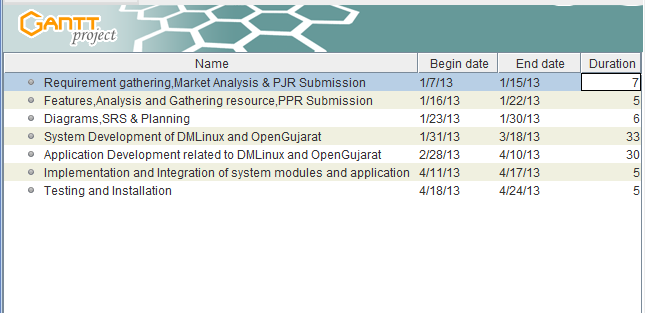
\includegraphics[scale=0.6] {gantt1.png}
  \caption[Project Planning]{Project Plan}
\end{center}
\end{figure}
\begin{figure}[h]
\begin{center}
  % Requires \usepackage{graphicx}
  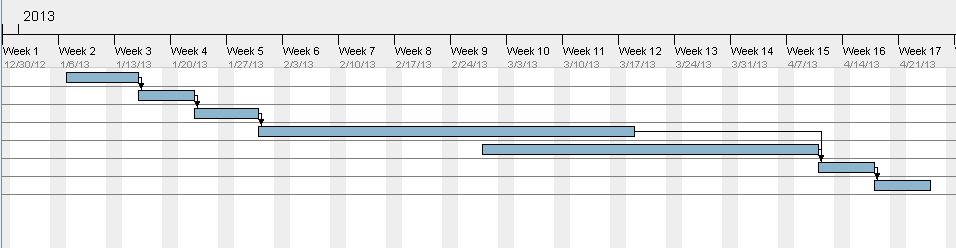
\includegraphics[scale=0.4] {gantt2.png}\\
  \caption[Timeline]{Project Plan - Timeline}
\end{center}
\end{figure}


\chapter{System Analysis}
\section{Feasibility Study}
The Objective of the Feasibility study:
The purpose of the Feasibility study is to find out if an information system project can be done and to suggest possible alternate solution. Feasibility study of the system is very important stage during the system design. Feasibility study is a test of a system proposal according to its workability impact on the organization, ability to meet user needs, and effective use of resources. (Hardware, Software, or other equipments), It is also use to determine whether the system gives benefit to people or society or not? Feasibility study decides whether the proposed system is properly developed or not or it properly work as per the expectation of the company or not.

Need for Feasibility Study:
A feasibility study is written approach to evaluating your idea and can help you identify:
\begin{itemize}
\item If your idea is viable or not
\item Useful facts and figures to aid decision-making
\item Alternative approaches and solutions to putting your idea into practice
\end{itemize}
There are many reasons why new community ventures fail, but lack of planning and research is the main one. As you plan, your knowledge of your market, customers and the environment in which you will work will grow. This process considers all areas of your idea and ensures you have something concrete on paper.

What does a feasibility study involve?

It can involve some or all of the following:
\begin{itemize}
\item An assessment of the current market
\item An assessment of your potential position in the market
\item An evaluation of the possible options for entry into the market
\item A short list of the possible options
\end{itemize}
There are some aspects in feasibility study portion of the preliminary investigation.
\begin{enumerate}
  \item Technical Feasibility.
  \item Economic Feasibility.
  \item Operational Feasibility.
  \item Social Feasibility.
  \item Legal Feasibility
  \item Time Feasibility of the project.
\end{enumerate}

\subsection{Technical feasibility}
A large part of determining resources has to do with assessing technical feasibility. It must be find out whether current technical resources can be upgraded or added in a manner that fulfills the request  under consideration. It is willing to improve its technical abilities of the project will be handled on the computerized concept so it has to improve some hardware and software abilities to maintain this system and it billing to improve and give all the supported facilities.
Here, the Proposed System which is to be developed requires Hardware as well as Software Resources.
A Hardware requirement includes PC with 40GB Hard disk and 1GB RAM.  Software requirement includes Java.
File requirement: Shape Files or geo referenced .jpg or .tiff file
It may be affordable for any organization to employee new professional thus, the requirement makes it technical feasible.

\subsection{Economic feasibility}
Economic feasibility looks at the financial aspects of the project. Economic feasibility concerns with the returns from the investments in a project. It determines whether it is worthwhile to invest the money in the proposed system. It is not worthwhile spending a lot of money on a project for no returns.
To carry out an economic feasibility for a system, it is necessary to place actual money value against any purchases or activities needed to implement the project.
The proposed system that is going to develop its benefit is indirect benefit and cost is direct cost that is to be paid. It costs for its development and hiring of the Server space. But it gives indirect benefit to businessman’s tourist etc.

\subsection{Operational feasibility}
The System will hold good GUI facilities which attract the user to use the System. The System will be developed using new technologies so the user will even get a chance work with and learn new technology and environment.
Company is having sufficient employees for designing, implementing, testing, deploying and the training the employee to uses that system.
In the system operational feasibility checks, whether the user who is going to use the system is able to work with the software’s with which the system is coded and also the mind of the user going to use the system. If the user does not understand or is able to work on the system further development is of waste.

\subsection{Social feasibility}
The System is going to be developed is it beneficial to society? Yes, as this System gives the details of the district to the user and admin and user can edit the shape files and get better view of the map also by having charts cam save as image which can be useful as map
\subsection{Legal feasibility}
The Proposed System should be such that the System do not misguide or gives wrong information to user. The System should give proper information and should be reliable source of information to user.
\subsection{Time feasibility}
The Proposed System is a Desktop  Application so it will take some duration of time to satisfy the objective of completing the System (Application). The duration that is allocated to develop the System is quite feasible in respect to time. 4 months is enough to develop System.

\section{Requirement Analysis}
\subsection{Facts finding techniques}
The client in most cases is not sure of what exactly is desired and has a poor understanding of the computing environment
\begin{itemize}
\item Inception of the Project
\item Basic Elicitation
\begin{itemize}
\item Problems of Scope
\item Problems of Understanding
\item Problems of Volatility
\end{itemize}
\item Elaboration
\item Negotiation
\item Specification
\item Validation
\item Management (Continuous)
\item The  following  techniques  are  present  unambiguously  throughout  the  project  and possess enormous power with regard to requirement gathering.
\end{itemize}

\subsubsection{Interview}
The requirement analysis phase begins after the inception of the project.
The first phase of interviews is mainly a kind of informal discussions with the client. In this phase the analysts who are the evangelists in the process of requirement elicitation generally do the following:
\begin{itemize}
\item Ask a set of Informal  Context Free Questions regarding  the system.
\item Talk   through   with   the   client   to   know   his   intention   with   regard   to   the project.
\item Define  a  business  case  for  the  idea  along  with  the  performance  of  certain kind of market analysis.
\item Identify a working description of the project’s scope.
\end{itemize}
The later phases of interviews involve the following kind of facets:
\begin{itemize}
\item Discussion  on  the  Division  of  the  entire  thing  into  manageable  and  doable modules.
\item Module wise interviews with the various personnel  involved.
\item Certain   kind   of   debatable   presentations   which   may   be   clubbed   with brainstorming or prototyping  sessions.
\end{itemize}
This mode of requirement gathering is the one that provides the maximum amount of information regarding the  project and hence is used very effectively. This mode can turn into all various forms ranging from strict one room interviews to large debatable discussions.

\subsubsection{Questionnaire}
This mode of requirement elicitation is generally employed during change management and while laying out basic system explanations.
Questionnaires used in the project are framed keeping into mind the following things:
\begin{itemize}
\item Amount and the kind  of information to be extracted  through this     channel.
\item The kind of stake holder to whom the questionnaire is addressed.
\item The reusability and  abstractness of these questionnaires.
\end{itemize}
\subsubsection{Record Review}

The records analyzed by me  were mainly the following:
\begin{itemize}
\item Software Design Document
This gave me the actual requirements of the GUI plus the backend logic right till statement of logical queries which may be employed in some or the other form. It also incorporated the sample GUI so that any  changes to the prototypes submitted earlier can be  checked and tracked.
\item Technical SRS (with Business Analysis)
This was a typical  SRS  that gave me the specific requirements along with the Business rules that need to be employed.
\item Class Diagrams
The class diagram made me understand the entire architecture that was employed and allowed me to extend it in my system.
\end{itemize}
\subsubsection{Observation}
This is also the method employed very widely in the project being developed. The  developers working   onsite generally engage in the observation of the following things:
\begin{itemize}
\item Work Environment of the organization.
\item The technical expertise of the employees of the organization.
\item The volume of customers entertained.
\item The kind of system expected.
\item The  resistance  in  the  organization  due   while   the   organization  gets   the system installed.
\item The usage of any of the available systems.
\end{itemize}
During the continuous management phase that starts once the system is installed and is running the   observation regarding system usage, system inconveniences and system benefits is carried  out.

\subsection{Data Flow Diagrams}
\begin{figure}[h]
\begin{center}
  % Requires \usepackage{graphicx}
  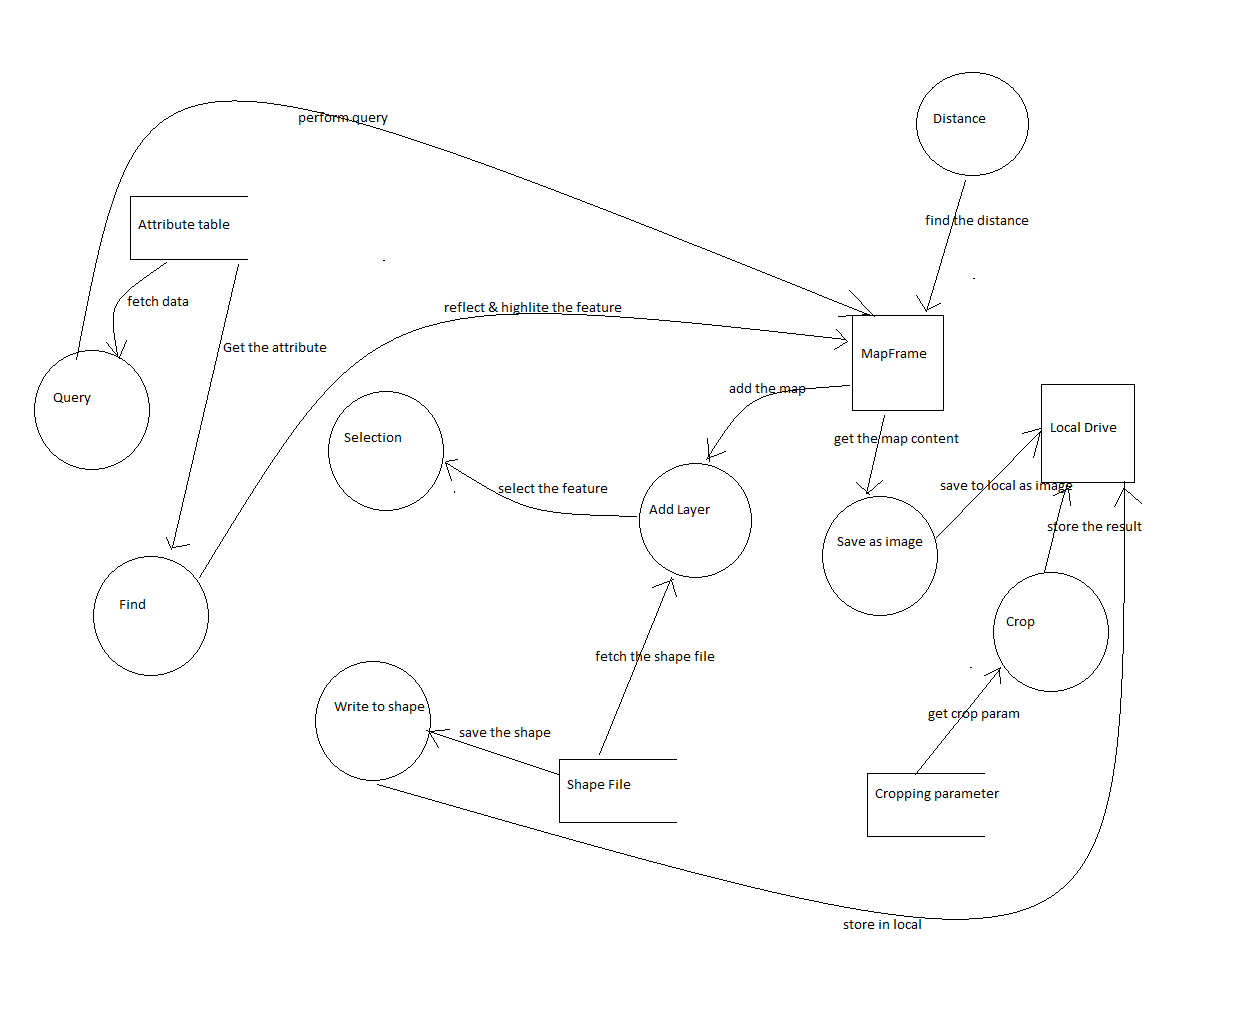
\includegraphics [scale=0.43] {DataFlow.png}
  \caption[Data Flow Diagram]{Data flow diagram of desktop GIS application}
\end{center}
\end{figure}

\chapter{System Diagram}
\begin{figure}[h]
\begin{center}
  % Requires \usepackage{graphicx}
  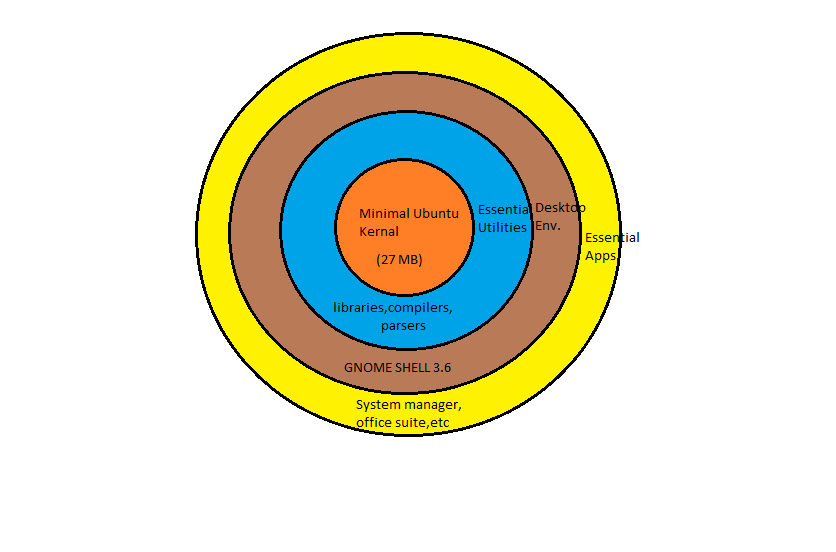
\includegraphics [scale=0.8] {core.png}
  \caption[System Ovierview]{Layered diagram of System}
\end{center}
\end{figure}
\begin{figure}[h]
\begin{center}
  % Requires \usepackage{graphicx}
  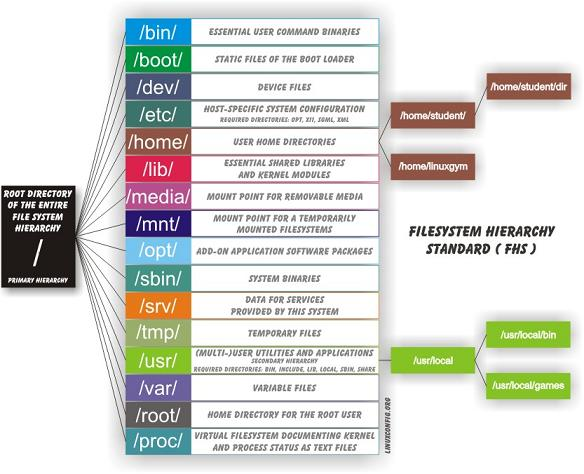
\includegraphics [scale=0.55] {dir.jpg}
  \caption[FIle system Diagram]{Linux File directories diagram}
\end{center}
\end{figure}

\chapter{Application Development}
We have developed some basic utilites that are going to enhance operating system experience.

\section{UTILITIES}
\begin{enumerate}

\item Auto ON Utility:\\
This application is developed with the aim of booting up PC at given time from shut down. This software is developed for Linux systems not for windows.
\begin{figure}[h]
\begin{center}
  % Requires \usepackage{graphicx}
  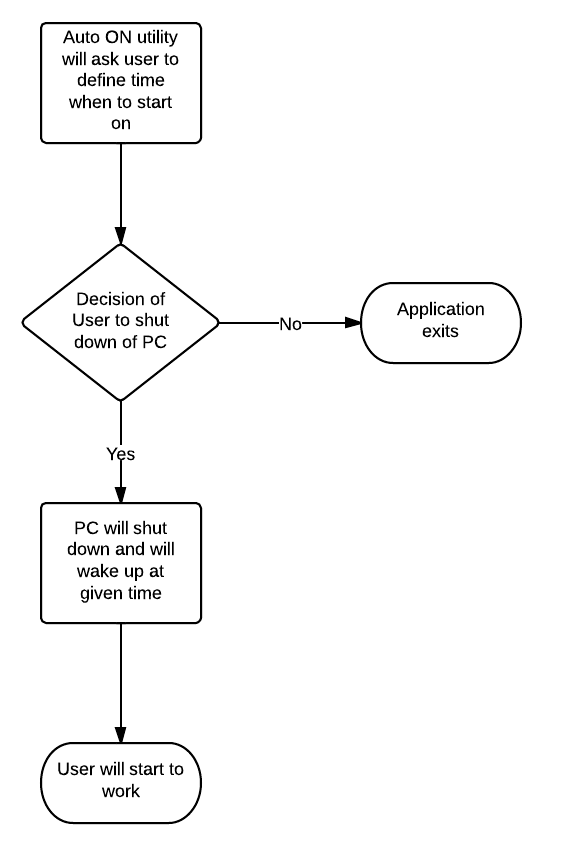
\includegraphics [scale=0.8] {aoutil.png}
  \caption[Auto ON Utility]{Auto ON Utility Flowchart}
\end{center}
\end{figure}

\item	LAMP(Front end)\\
This application is developed with the aim to handle LAMP Services(Apache, MySQL and PHP Services installed inside Linux system)

\item Repocloner\\
Repocloner is an application to make local apt repository for intranet based servers.
This application is for server side which has linux installed.
\item	Multidoc Converter\\
This application is developed with aim to convert multiple document formats between each other. 
\end{enumerate}

\section{Gujarati Dictionary}
\subsection {Purpose}
	This dictionary is general dictionary that will provide meaning of given English words into gujarati meaning.
	Dictionary is going to develop for OpenGujarat as well as this dictionary can be ported or installed in other system.
\subsection{Current Alternative Application}
	There is no dictionary (English to Gujarati) available for any linux(debian or RPM package management system) operating system till now. 
	This is our first time development in this space.

\subsection{Porting System}
We will try to port this dictionary on multiple platform in short time.
We have short time so we will try to use other third party application to port our dictionary in desired system.
Our dictionary can be insalled on Windows,Mac OS X,Android and Linux system.
\subsection{Component of Dictionary Development}
\subsubsection{Dictionary Front End}
	Dictionary front end means Dicitonary look up program. The application that gives interface between database and user to manipulate information in easy way.

\begin{itemize}
\item LINUX :\\
STAR DICT (APPLICATION)  or GOLDEN DICT(APPLICATION):\\
This front end application is available on Ubuntu repository. You can install via following commands.

\item	ANDROID:\\
Golden Dict(Application):\\
This front end application can be downloaded from Google play store.(Link)

\end{itemize}	
	\subsection{Dictionary back end}
Dictionary back end means the database that includes English words and meaning of that words in Gujarati.
	Database is provided by GujaratiLexicon.com.
	This database contains around 52,000 words.

\chapter{Class Diagram and CRC card}

\section{Class Diagram}

\begin{figure}[h]
\begin{center}
  % Requires \usepackage{graphicx}
  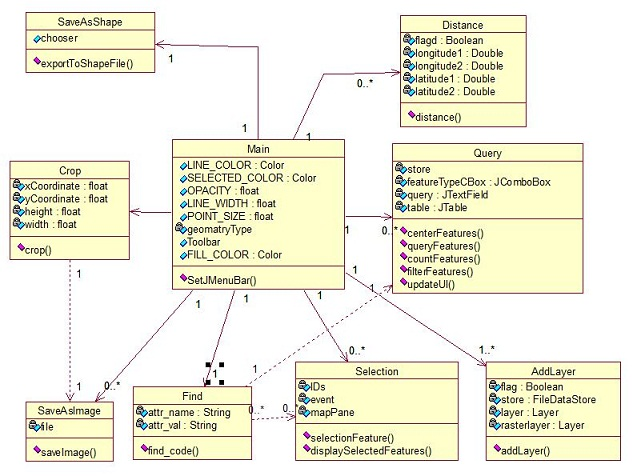
\includegraphics[scale=0.8] {Class.jpg}
  \caption [Class Diagram]{class diagram of entire system}
\end{center}
\end{figure}

\section{CRC Index Card}

\begin{table}[h]
\begin{tabular}{|p{7cm}|p{7cm}|}
  \hline
  % after \\: \hline or \cline{col1-col2} \cline{col3-col4} ...
  \multicolumn{2}{|l|}{ Class Name : Main} \\
  \hline
  \multicolumn{2}{|l|}{ Class Type : interaction, connection} \\
  \hline
  \multicolumn{2}{|l|}{ Class Characteristics : secure, sequential, permanent} \\
  \hline
  Responsibilities & Collaborators  \\
  \hline
  Create main window & Selection \\
  Open layers & Find \\
   & Save as Image\\
   & Crop \\
   & Add Layer \\
   & Query \\
   & Distance \\
  \hline
\end{tabular}
\caption[CRC card - Main Class]{CRC card - Main}
\end{table}

\begin{table}[h]
\begin{tabular}{|p{7cm}|p{7cm}|}
  \hline
  % after \\: \hline or \cline{col1-col2} \cline{col3-col4} ...
  \multicolumn{2}{|l|}{ Class Name :   Selection} \\
  \hline
  \multicolumn{2}{|l|}{ Class Type : interaction, connection} \\
  \hline
  \multicolumn{2}{|l|}{ Class Characteristics : secure, sequential, temporary} \\
  \hline
  Responsibilities & Collaborators  \\
  \hline
  Make selection of raster file & Find \\
  Make selection of vector file & \\
  \hline
\end{tabular}
\caption[CRC card - Selection]{CRC card - Selection}
\end{table}

\begin{table}[h]
\begin{tabular}{|p{7cm}|p{7cm}|}
  \hline
  % after \\: \hline or \cline{col1-col2} \cline{col3-col4} ...
  \multicolumn{2}{|l|}{ Class Name : Query} \\
  \hline
  \multicolumn{2}{|l|}{ Class Type : interaction, connection} \\
  \hline
  \multicolumn{2}{|l|}{ Class Characteristics : secure, sequential, temporary} \\
  \hline
  Responsibilities & Collaborators  \\
  \hline
  Get feature from Layer  & Main\\
  Apply query on feature & \\
  \hline
\end{tabular}
\caption[CRC card - Query]{CRC card - Query}
\end{table}

\begin{table}[h]
\begin{tabular}{|p{7cm}|p{7cm}|}
  \hline
  % after \\: \hline or \cline{col1-col2} \cline{col3-col4} ...
  \multicolumn{2}{|l|}{ Class Name : Save as Shape} \\
  \hline
  \multicolumn{2}{|l|}{ Class Type : interaction, device} \\
  \hline
  \multicolumn{2}{|l|}{ Class Characteristics : secure, sequential, permanent} \\
  \hline
  Responsibilities & Collaborators  \\
  \hline
  Get the name of layer & jMapFrame \\
  Get the name of selected feature & jLayerTable \\
  Get name of new layer & \\
  Read the content of selected attribute & \\
  Write the content into new layer & \\
  \hline
\end{tabular}
\caption[CRC card - Save as Shape]{CRC card - Save as Shape}
\end{table}

\begin{table}[h]
\begin{tabular}{|p{7cm}|p{7cm}|}
  \hline
  % after \\: \hline or \cline{col1-col2} \cline{col3-col4} ...
  \multicolumn{2}{|l|}{ Class Name : Save as Image} \\
  \hline
  \multicolumn{2}{|l|}{ Class Type : interaction, device} \\
  \hline
  \multicolumn{2}{|l|}{ Class Characteristics : secure, sequential, permanent} \\
  \hline
  Responsibilities & Collaborators  \\
  \hline
  Get the name of layer & \\
  Get the content of mapframe & \\
  Get name of new imagefile & \\
  Read the content of frame & \\
  Write the content into local file as image & \\
  \hline
\end{tabular}
\caption[CRC card - Save as Image]{CRC card - Save as Image}
\end{table}

\begin{table}[h]
\begin{tabular}{|p{7cm}|p{7cm}|}
  \hline
  % after \\: \hline or \cline{col1-col2} \cline{col3-col4} ...
  \multicolumn{2}{|l|}{ Class Name : Distance} \\
  \hline
  \multicolumn{2}{|l|}{ Class Type : interaction, connection} \\
  \hline
  \multicolumn{2}{|l|}{ Class Characteristics : secure, sequential, permanent} \\
  \hline
  Responsibilities & Collaborators  \\
  \hline
  Get the points & Main \\
  Apply the algorithm & \\
  Display result in Km. & \\
  \hline
\end{tabular}
\caption[CRC card - Distance]{CRC card - Distance}
\end{table}

\begin{table}[t]
\begin{tabular}{|p{7cm}|p{7cm}|}
  \hline
  % after \\: \hline or \cline{col1-col2} \cline{col3-col4} ...
  \multicolumn{2}{|l|}{ Class Name : Crop} \\
  \hline
  \multicolumn{2}{|l|}{ Class Type : interaction, connection, device} \\
  \hline
  \multicolumn{2}{|l|}{ Class Characteristics : secure, sequential, permanent} \\
  \hline
  Responsibilities & Collaborators  \\
  \hline
  Get the cropping parameter & Main \\
  Save the temporary result in image & save as image \\
  Crop that image & \\
  Save the Cropped result in Local file & \\
  \hline
\end{tabular}
\caption[CRC card - Crop]{CRC card - Crop}
\end{table}

\chapter{User Manuals}

\begin{figure}[h]
\begin{center}
  % Requires \usepackage{graphicx}
  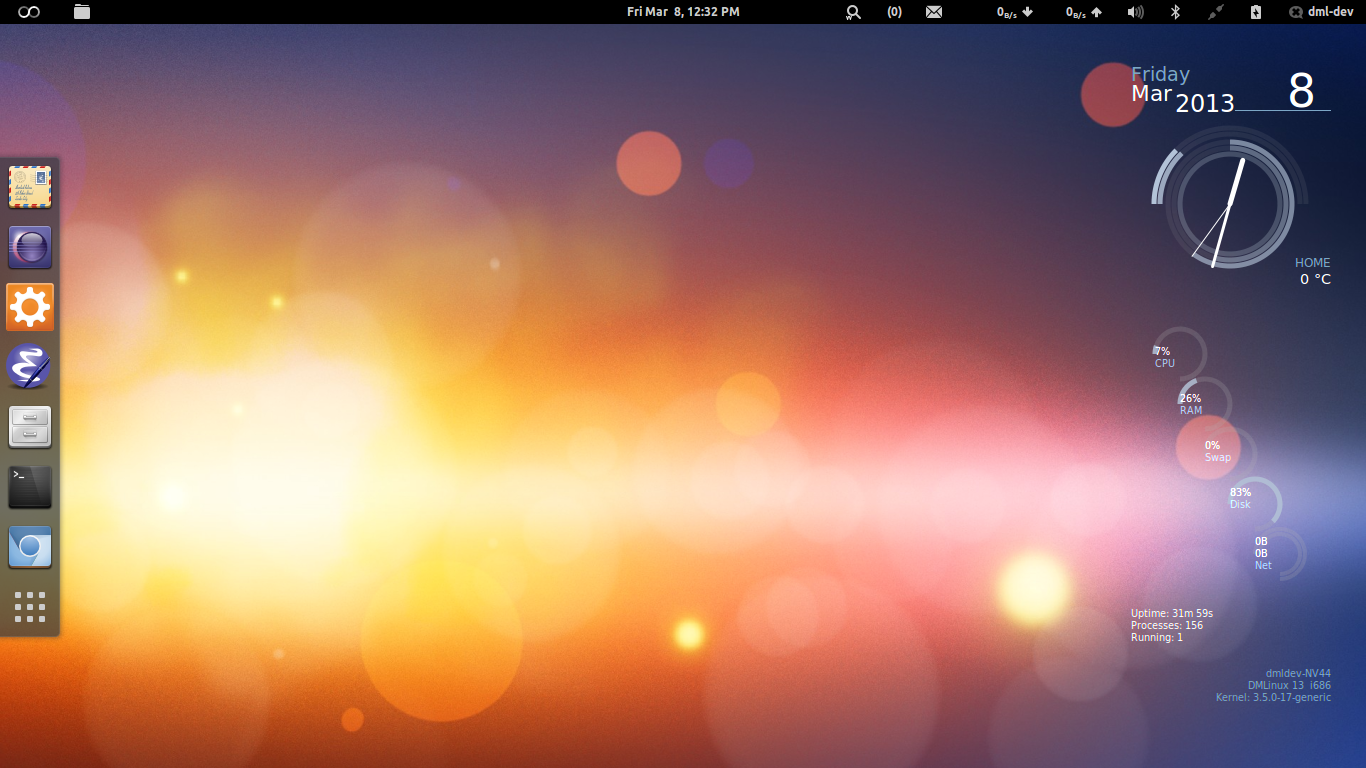
\includegraphics[scale=0.35] {1.png}
  \caption[Screenshot - DMLinux Main Desktop]{Main outlook of DMLinux}
\end{center}
\end{figure}
Description: Above is the Desktop of DMLinux Operating system.It feature GNOME Shell 3.6 inside it.Theme and icons are added by us.

\newpage
\begin{figure}[h]
\begin{center}
  % Requires \usepackage{graphicx}
  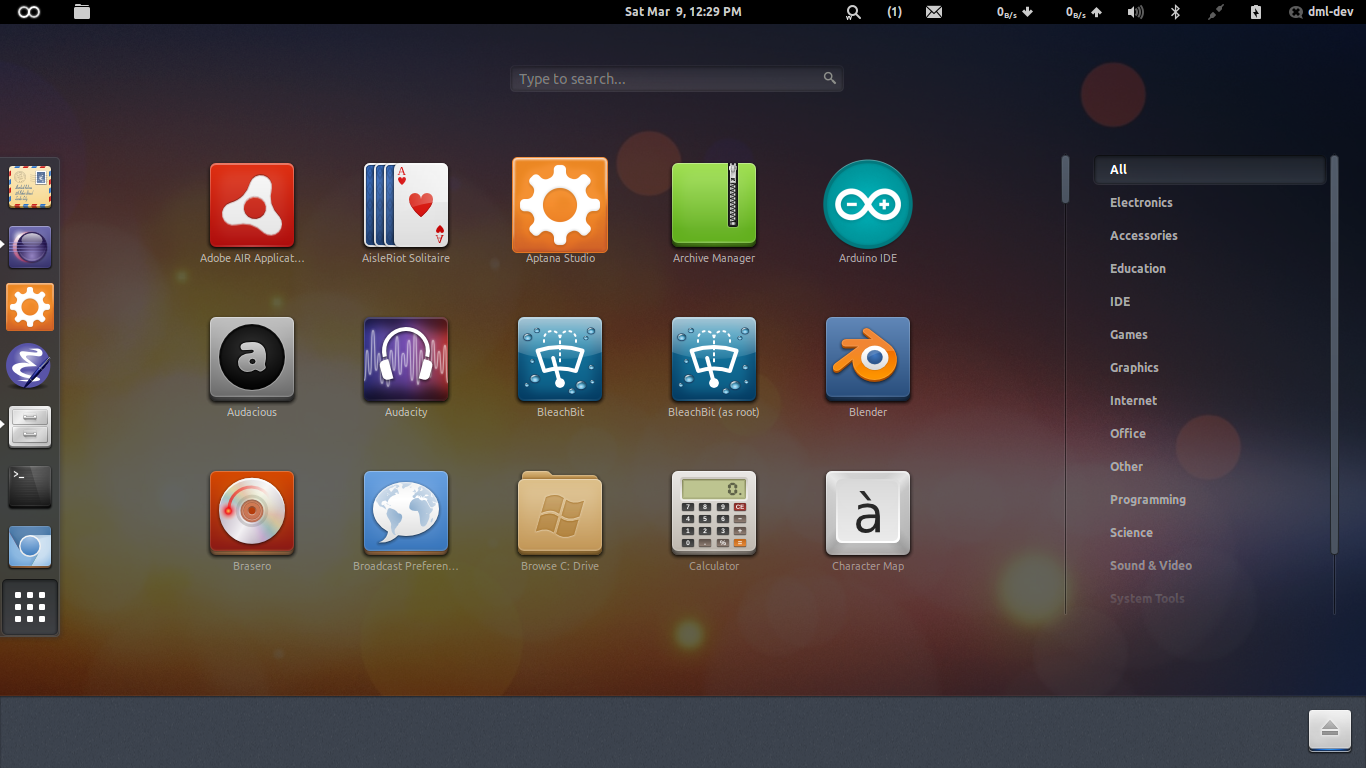
\includegraphics[scale=0.35] {2.png}
  \caption[Screenshot - Application Menu]{Application Menu}
\end{center}
\end{figure}
Description: Above is the screenshot of Application Menu provided in DMLinux .It offeres catogary wise application list.

\newpage
\begin{figure}[h]
\begin{center}
  % Requires \usepackage{graphicx}
  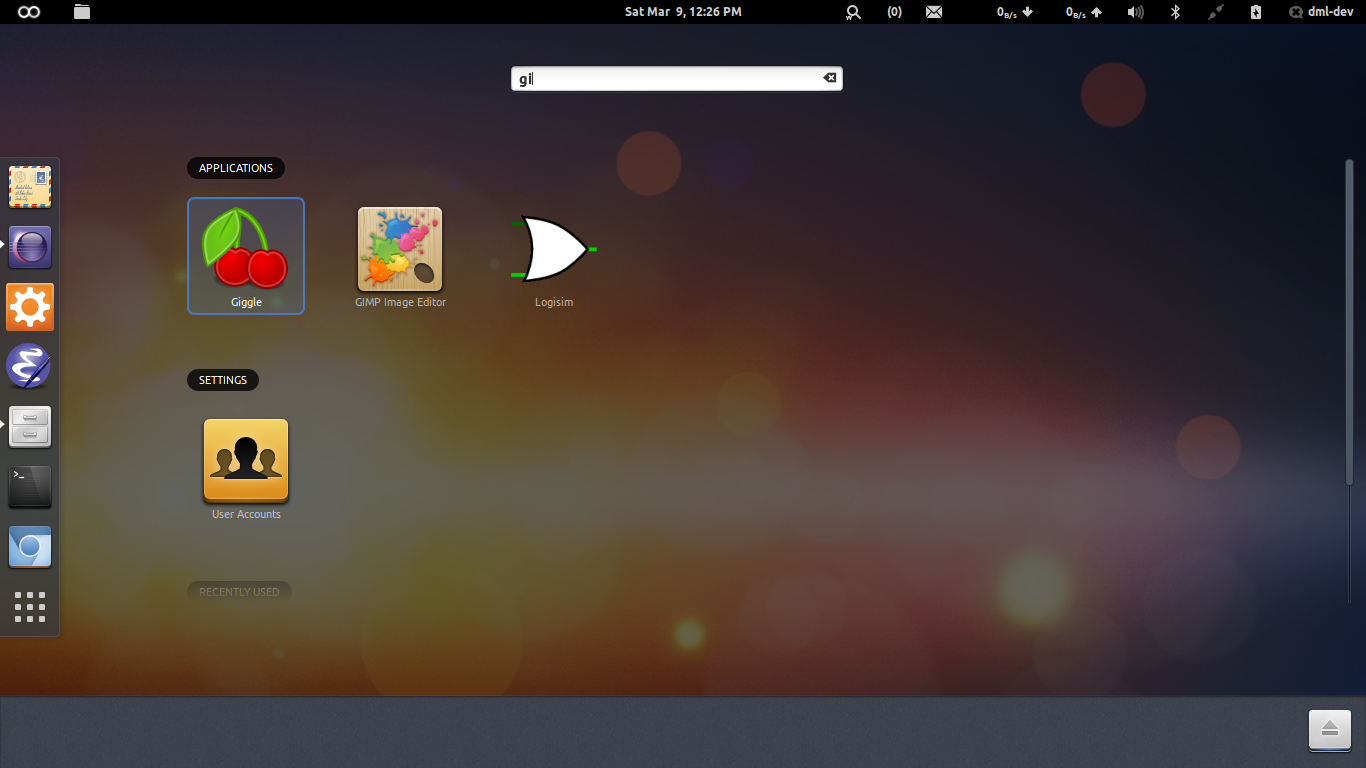
\includegraphics[scale=0.35] {3.png}
  \caption[Screenshot - Search Dash in DMLinux]{Search Dash}
\end{center}
\end{figure}
Description: By pressing Windows Key, User enters in search dash. Here user can search any application,files,settings etc in installed system.

\newpage


\begin{figure}[h]
\begin{center}
  % Requires \usepackage{graphicx}
  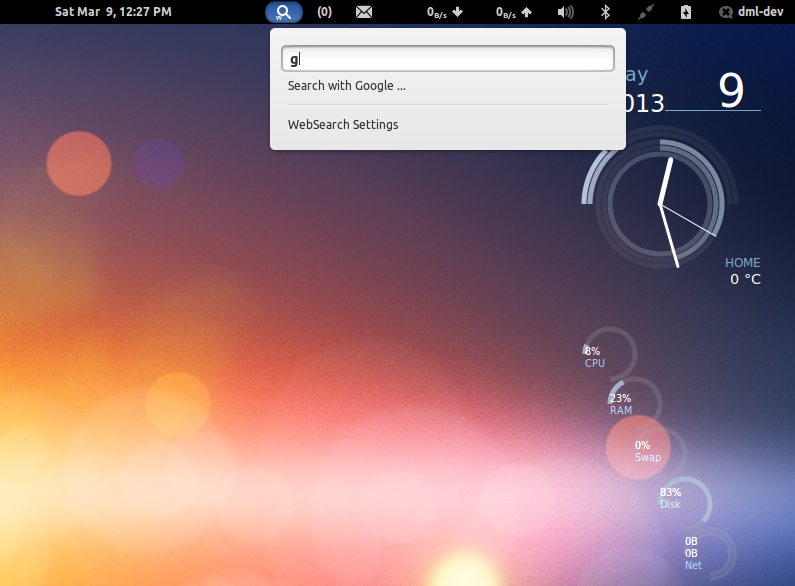
\includegraphics[scale=0.4] {4.png}
  \caption[Screenshot - Web search Applet]{Inbuilt Web Search Applet}
\end{center}
\end{figure}
Description: It is useful applet attached with top panel.User can search on web sites like google and wikipedia directly from here.

\newpage
\begin{figure}[h]
\begin{center}
  % Requires \usepackage{graphicx}
  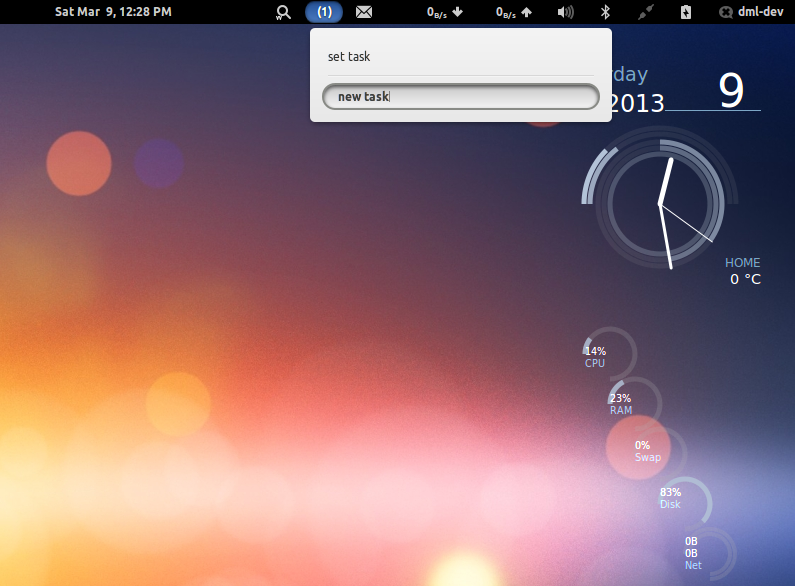
\includegraphics[scale=0.4] {5.png}
  \caption[Screenshot - To-do list applet]{Inbuilt To-do task applet}
\end{center}
\end{figure}
Description: It is useful applet attached with top panel.User can make to-do list of everday' task and whenever its completed,he/she can delete it by clicking on that task.
\newpage
\begin{figure}[h]
\begin{center}
  % Requires \usepackage{graphicx}
  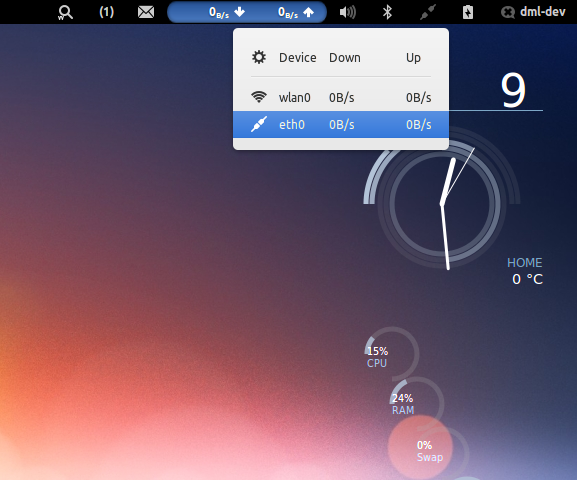
\includegraphics[scale=0.4] {6.png}
  \caption[Screenshot - Network Meter]{Network Meter}
\end{center}
\end{figure}
Description: It is a live network monitor attached with top panel.User can see the speed of network via this applet.

\newpage
\begin{figure}[h]
\begin{center}
  % Requires \usepackage{graphicx}
  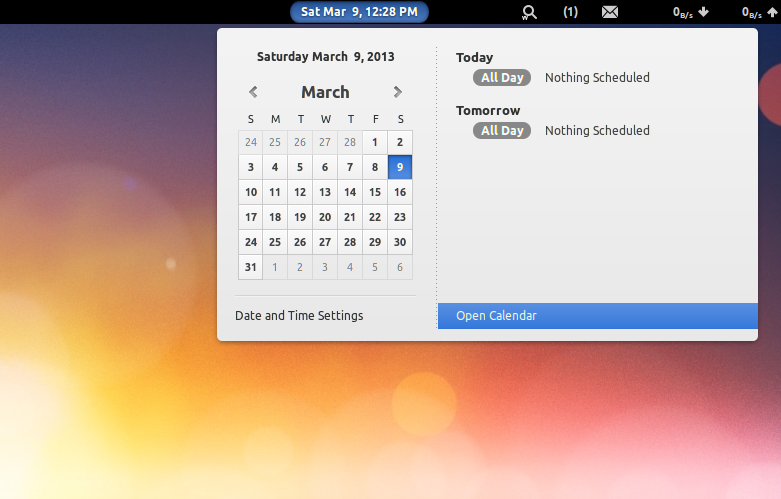
\includegraphics[scale=0.4] {7.png}
  \caption[Screenshot - Calender applet]{Calendar support}
\end{center}
\end{figure}
Description: Above feature is useful to plan a task or month using calendar on Evolution Mail client.It is handy tool with top panel for plainnig big task or any important task.

\newpage

\begin{figure}[h]
\begin{center}
  % Requires \usepackage{graphicx}
  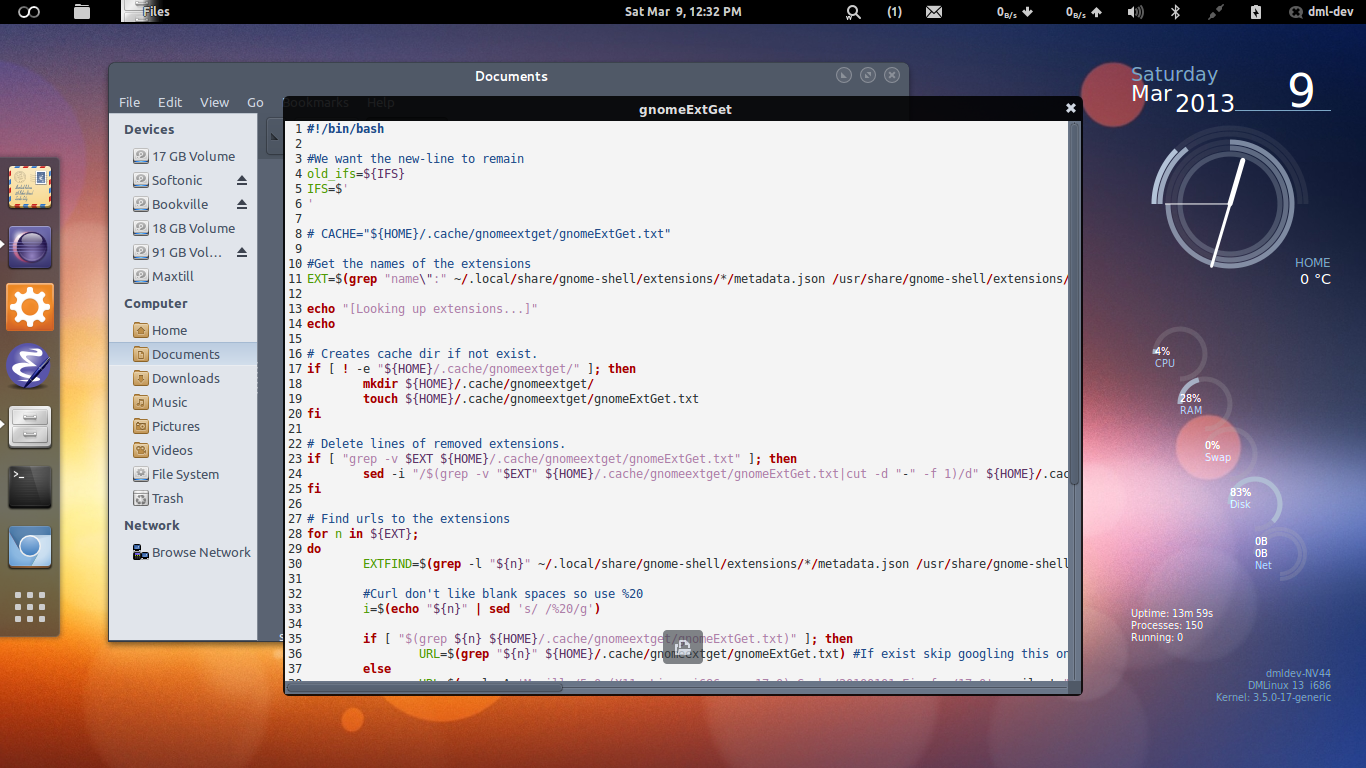
\includegraphics[scale=0.35] {8.png}
  \caption[Screenshot - Quick Preview]{Quick Preview support}
\end{center}
\end{figure}
Description: User can see the preview of txt,folders,pdf,image,music and video files directly by pressing SPACE BAR on the file in file manager.It is useful feature of GNOME Shell 3.6.
\newpage
\begin{figure}[h]
\begin{center}
  % Requires \usepackage{graphicx}
  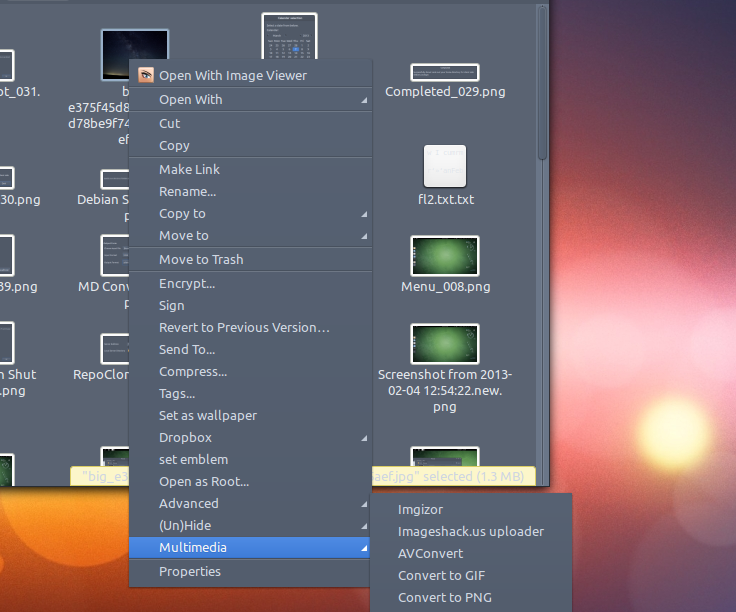
\includegraphics[scale=0.4] {9.png}
  \caption[Screenshot - Extended Right Menu]{Extended right menu}
\end{center}
\end{figure}
Description : Extended right menu provides lots of feature that can be directly performed on file or folder via clicking right mouse button.It has handsfull features like image resizing,hide/unhide,checksum,dropbox sharing etc.It is nautilus extra package provided in the system.
\newpage
\begin{figure}[h]
\begin{center}
  % Requires \usepackage{graphicx}
  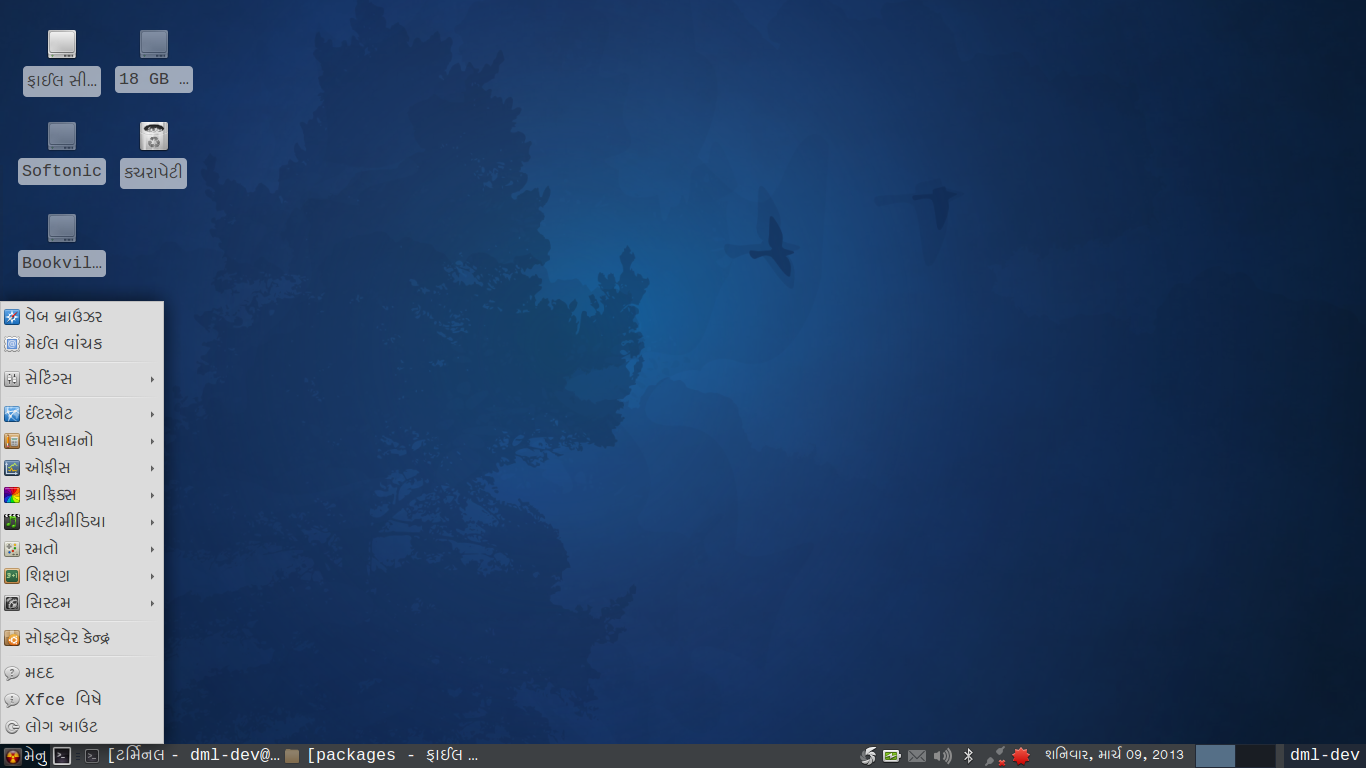
\includegraphics[scale=0.35] {10.png}
  \caption[Screenshot - OpenGujarat Main Desktop]{OpenGujarat Main Desktop View}
\end{center}
\end{figure}
Description: This is a screenshot of OpenGujarat OS Main Desktop View.It contains XFCE 4.1 Desktop Environment.It is designed as windows type mock up by us.
\newpage


\begin{figure}[h]
\begin{center}
  % Requires \usepackage{graphicx}
  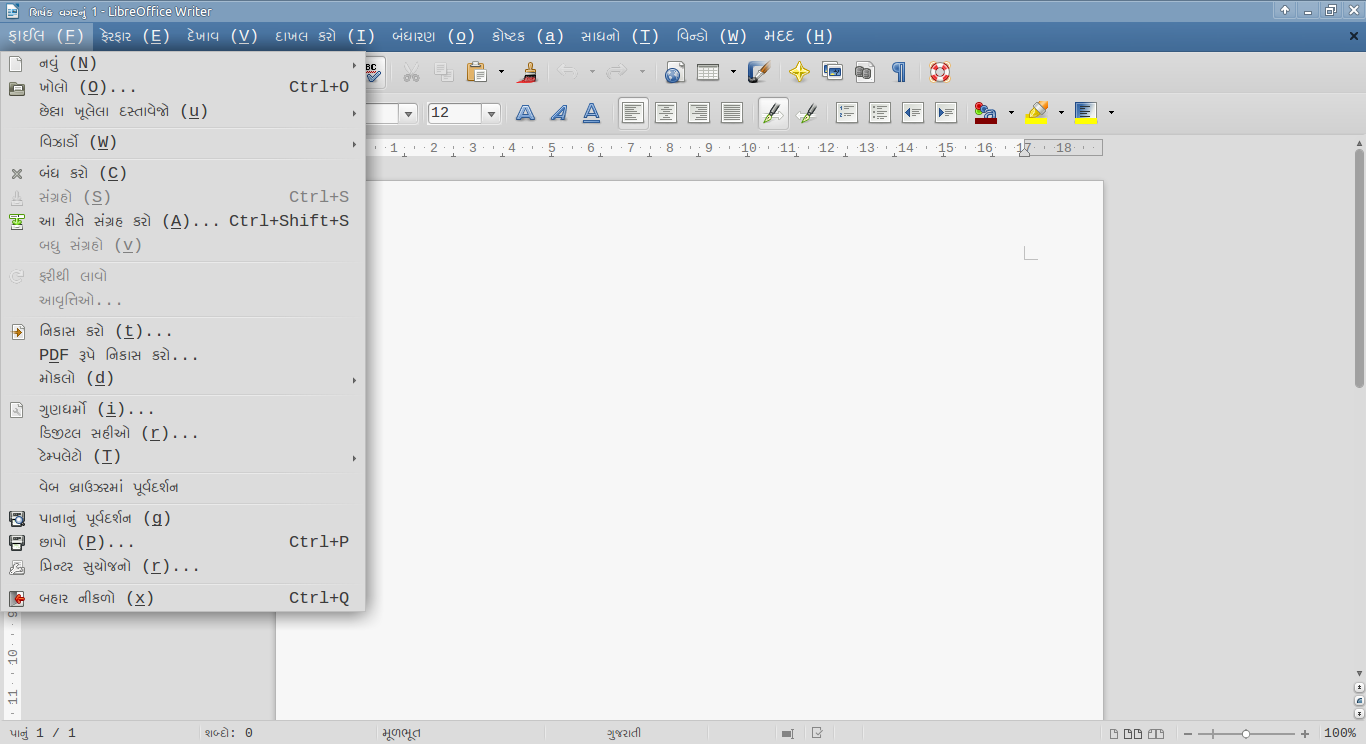
\includegraphics[scale=0.35] {11.png}
  \caption[Screenshot - Office suite in Gujarati]{LibreOffice suite in Gujarati}
\end{center}
\end{figure}
Description: Above is screenshot of LibreOffice suite inbuilt in OpenGujarat OS.

\newpage
\begin{figure}[h]
\begin{center}
  % Requires \usepackage{graphicx}
  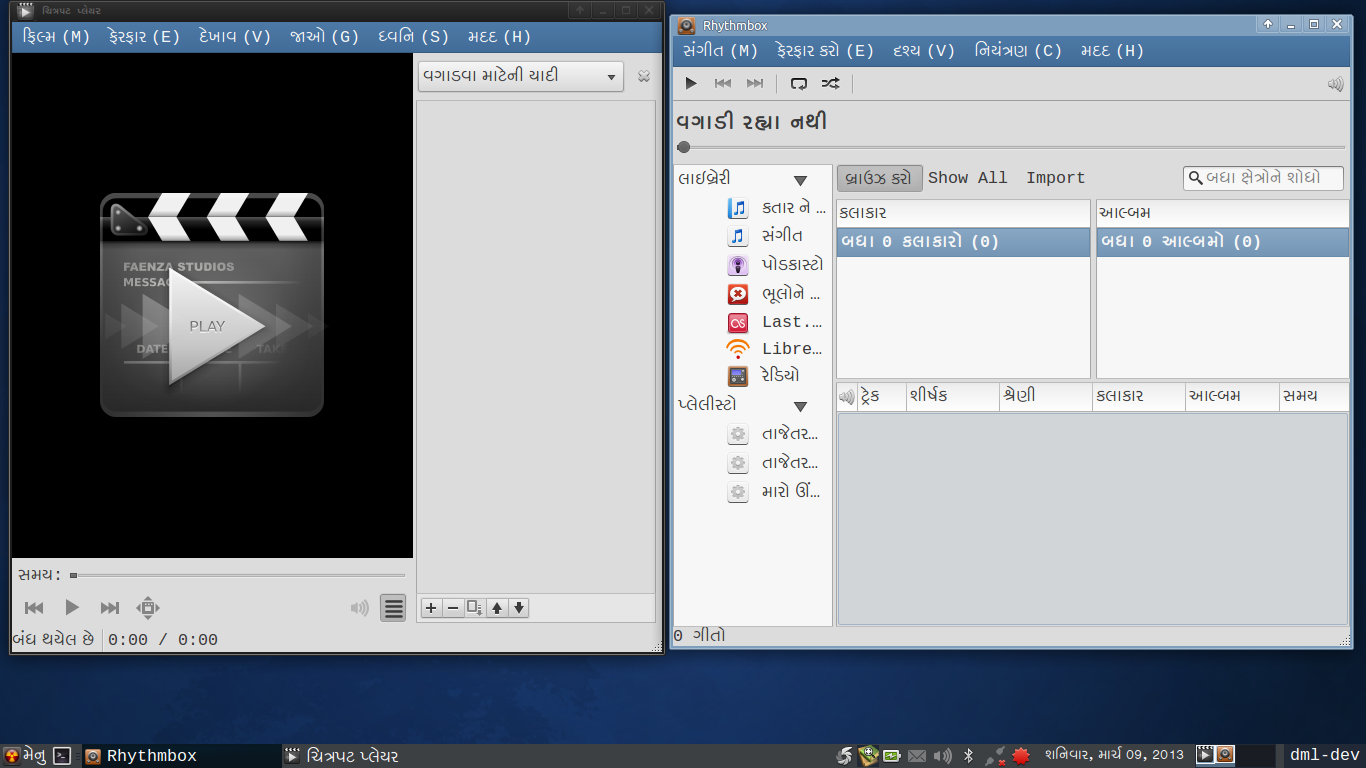
\includegraphics[scale=0.35] {12.png}
  \caption[Screenshot - Music and Media player in OpenGujarat]{Music and Media Player in Gujarati}
\end{center}
\end{figure}
Description:  Above is screenshot of Music and Media player inbuilt in OpenGujarat OS.

\newpage

\begin{figure}[h]
\begin{center}
  % Requires \usepackage{graphicx}
  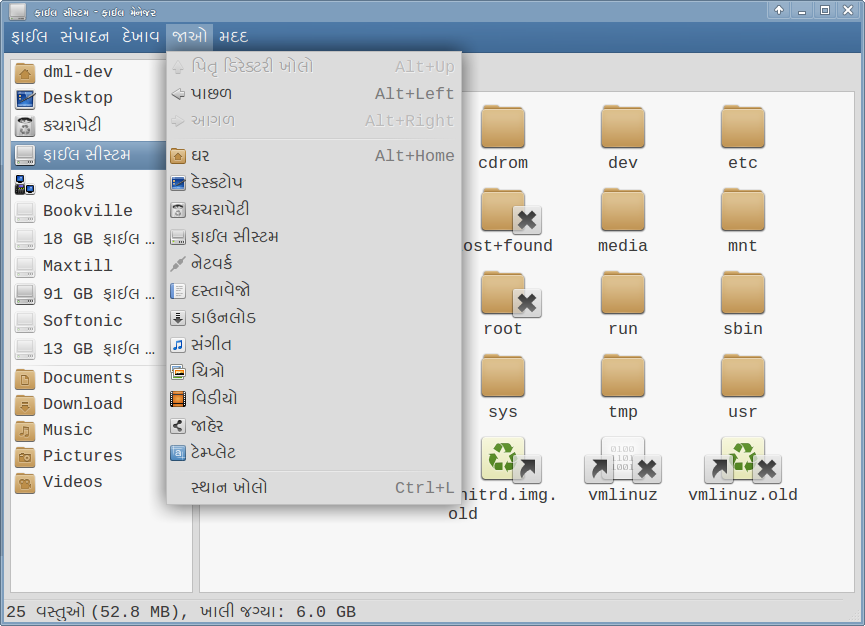
\includegraphics[scale=0.4] {13.png}
 \caption[Screenshot - Thunar File manager]{Thunar File manager}
\end{center}
\end{figure}
Description: It is screenshot of thunar file manager translated in gujarati provided in OpenGujarat.

\newpage
\begin{figure}[h]
\begin{center}
  % Requires \usepackage{graphicx}
  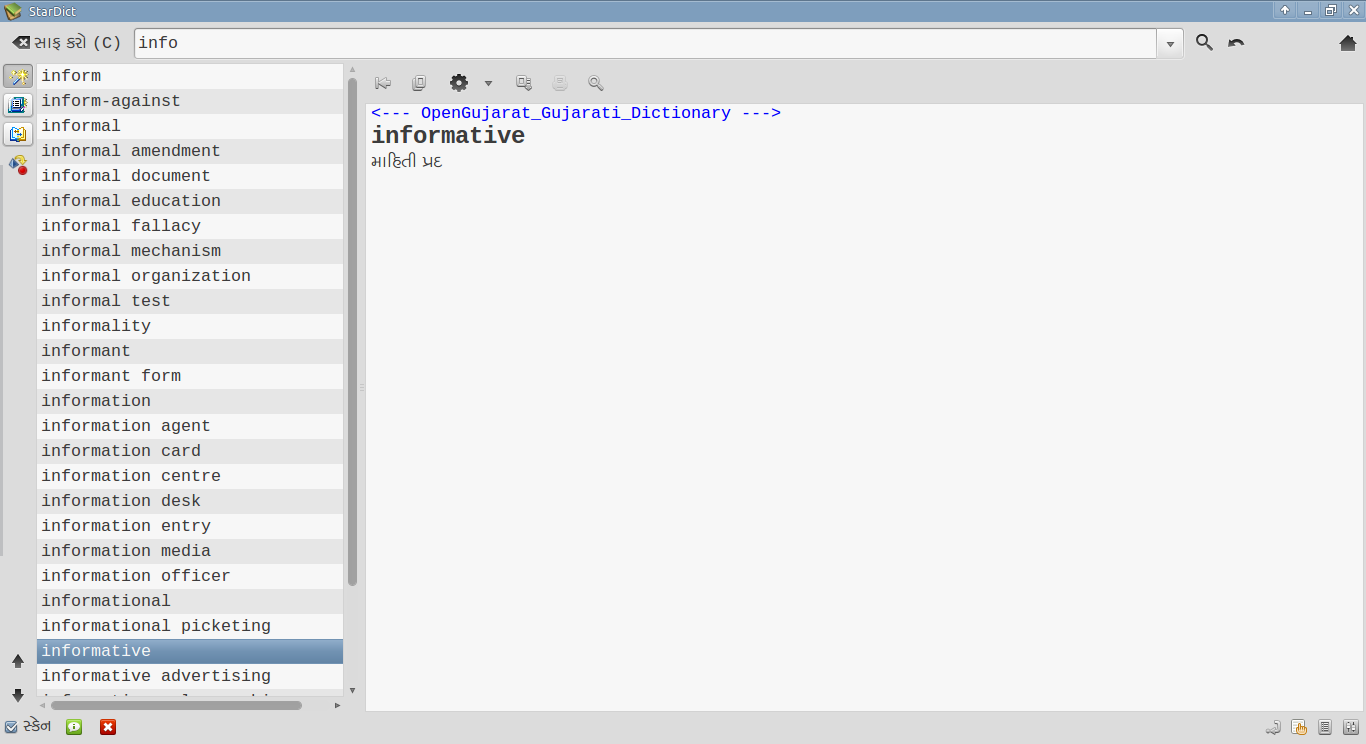
\includegraphics[scale=0.4] {14.png}
  \caption[Screenshot - Gujarati Dictionary]{Gujarati Dictionary Main View}
\end{center}
\end{figure}
Description: It is main search bar of Gujarati dictionary with stardict dictionary look up program.
\newpage

\begin{figure}[h]
\begin{center}
  % Requires \usepackage{graphicx}
  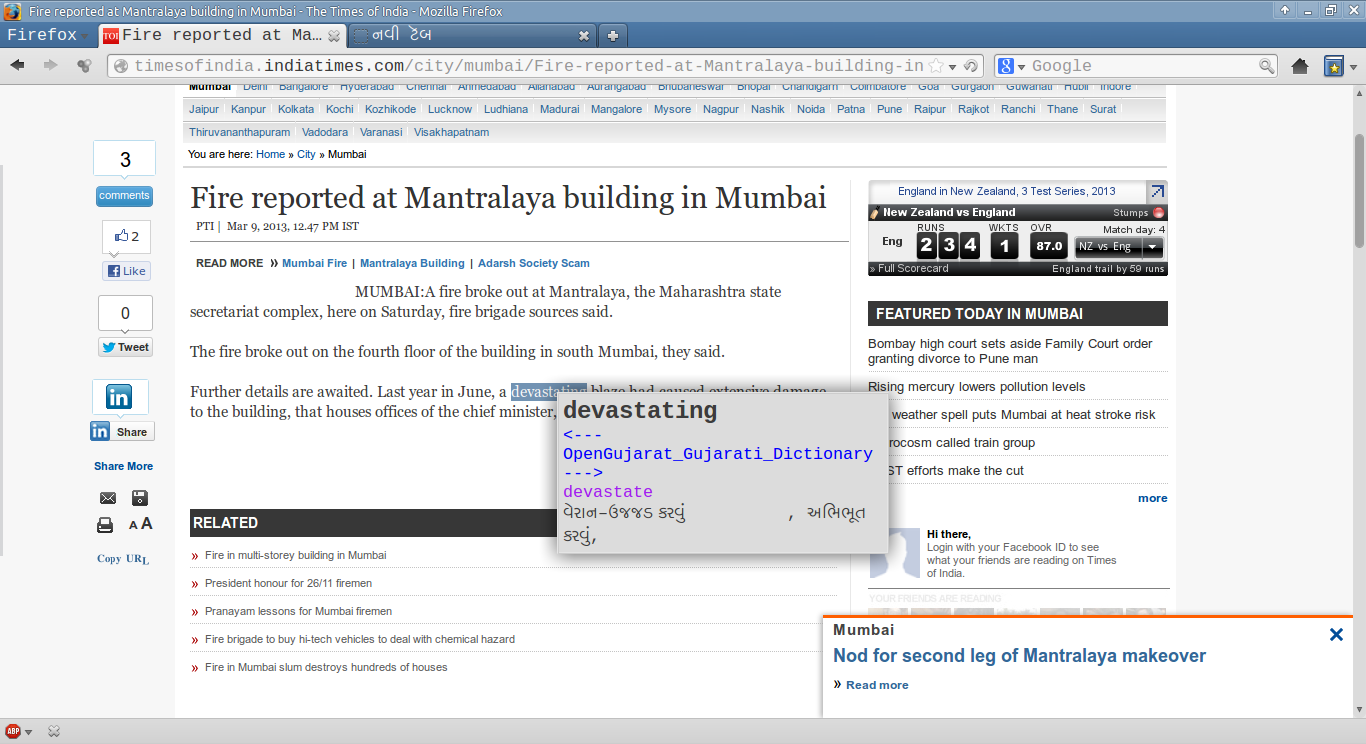
\includegraphics[scale=0.35] {15.png}
  \caption[Screenshot - Gujarati Dictionary Live search]{Gujarati Dictionary Live search}
\end{center}
\end{figure}
Description: Here is the output as dialog box clicked on the word to get the meaning of English word in Gujarati dictionary.Result is provided by Stardict application as pop up box.

\newpage
\begin{figure}[h]
\begin{center}
  % Requires \usepackage{graphicx}
  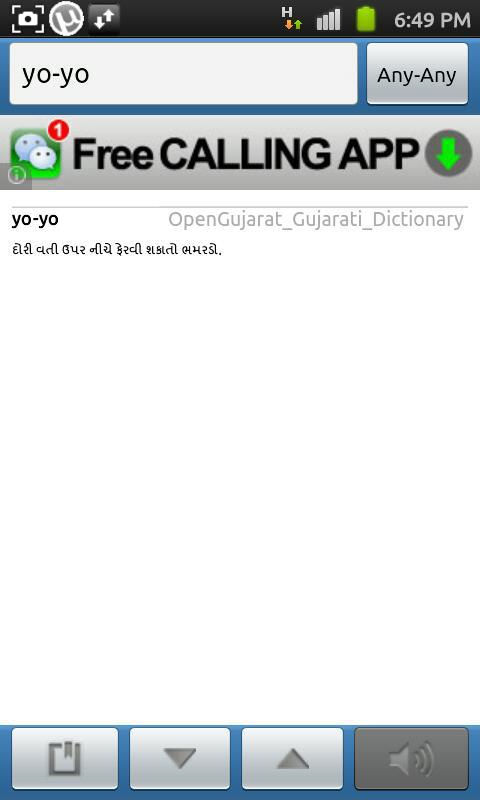
\includegraphics[scale=0.67] {16.png}
  \caption[Screenshot - Gujarati Dictionary Android View]{Gujarati Dictionary Android View}
\end{center}
\end{figure}
Description: It is a screenshot of Gujarati dictionary ported to android phone via GoldenDict Dictionary Look up program.
\newpage
\begin{figure}[h]
\begin{center}
  % Requires \usepackage{graphicx}
  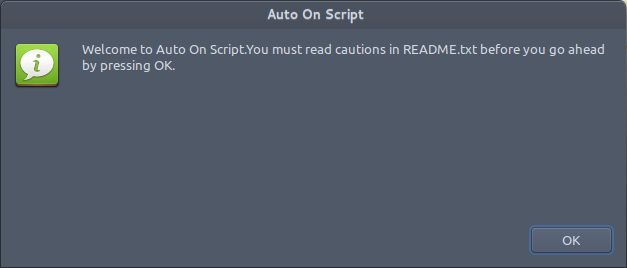
\includegraphics[scale=0.65] {17.png}
  \caption[Screenshot - Auto ON Utility Start Up screen]{Auto ON Utility Start Up screen}
\end{center}
\end{figure}
Description: Here is the start up screen of auto on utility .
\begin{figure}[h]
\begin{center}
  % Requires \usepackage{graphicx}
  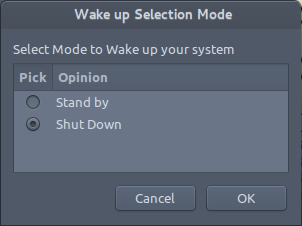
\includegraphics[scale=0.79] {18.png}
  \caption[Screenshot - Mode selection in Auto ON Utility]{Mode selection in Auto ON Utility}
\end{center}
\end{figure}
Description: User have to select in which mode he/she wants to boot pc after given time.

\begin{figure}[h]
\begin{center}
  % Requires \usepackage{graphicx}
  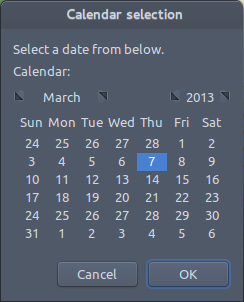
\includegraphics[scale=0.79] {19.png}
  \caption[Screenshot - Date Selection]{Date selection}
\end{center}
\end{figure}

\begin{figure}[h]
\begin{center}
  % Requires \usepackage{graphicx}
  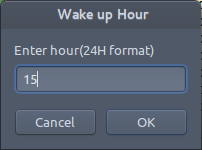
\includegraphics[scale=0.99] {20.png}
  \caption[Screenshot - Hour Entry Box]{Hour Entry Box}
\end{center}
\end{figure}
\begin{figure}[h]
\begin{center}
  % Requires \usepackage{graphicx}
  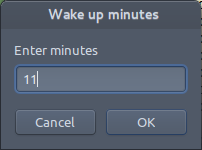
\includegraphics[scale=0.99] {21.png}
  \caption[Screenshot - Minutes Entry Box]{Minutes Entry Box}
\end{center}
\end{figure}\begin{figure}[h]
\begin{center}
  % Requires \usepackage{graphicx}
  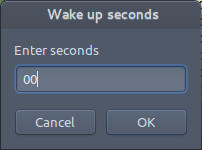
\includegraphics[scale=0.99] {22.png}
  \caption[Screenshot - Seconds Entry Box]{Seconds Entry Box}
\end{center}
\end{figure}

\begin{figure}[h]
\begin{center}
  % Requires \usepackage{graphicx}
  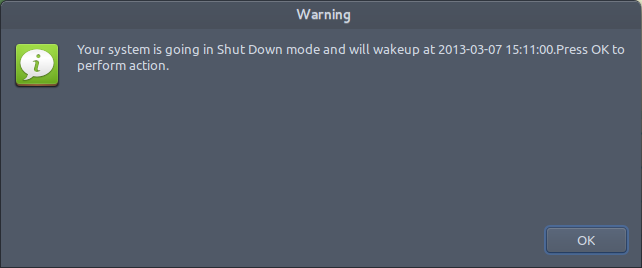
\includegraphics[scale=0.69] {23.png}
  \caption[Screenshot - Final warning of Auto ON Utility]{Final warning of Auto ON Utility}
\end{center}
\end{figure}

\begin{figure}[h]
\begin{center}
  % Requires \usepackage{graphicx}
  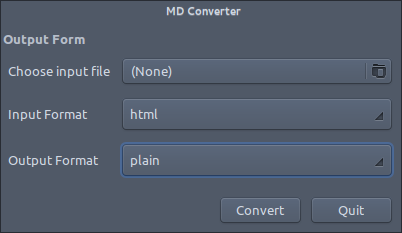
\includegraphics[scale=0.89] {24.png}
  \caption[Screenshot - MDConverter Main Screen]{Main Screen of MDCoverter}
\end{center}
\end{figure}
\begin{figure}[h]
\begin{center}
  % Requires \usepackage{graphicx}
  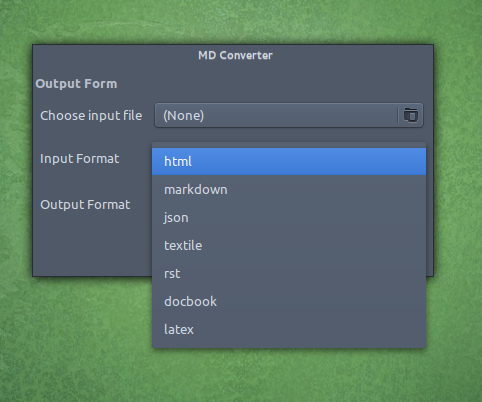
\includegraphics[scale=0.89] {25.png}
  \caption[Screenshot - MDConverter Input Options]{MDConverter Input Options}
\end{center}
\end{figure}
\begin{figure}[h]
\begin{center}
  % Requires \usepackage{graphicx}
  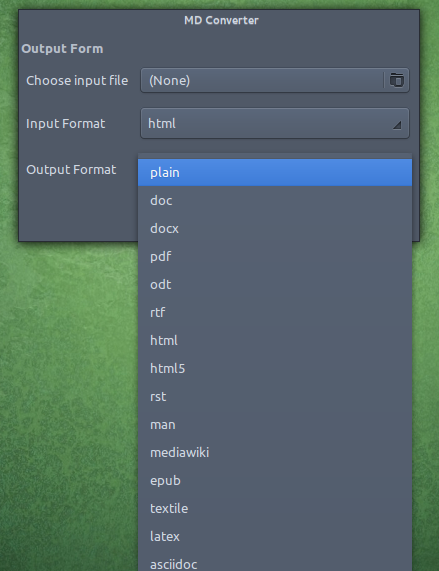
\includegraphics[scale=0.89] {26.png}
  \caption[Screenshot - MDConverter Output Options]{MDConverter Output Options}
\end{center}
\end{figure}
\newpage
\begin{figure}[h]
\begin{center}
  % Requires \usepackage{graphicx}
  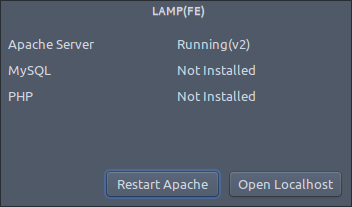
\includegraphics[scale=0.89] {27.png}
  \caption[Screenshot - LAMP Front End]{LAMP Front end Main Screen}
\end{center}
\end{figure}
\begin{figure}[h]
\begin{center}
  % Requires \usepackage{graphicx}
  
\includegraphics[scale=0.69] {28.png}
  \caption[Screenshot - LAMP Apache Server Restart Notification]{LAMP Apache Server Restart Notification}
\end{center}
\end{figure}
\newpage
\begin{figure}[h]
\begin{center}
  % Requires \usepackage{graphicx}
  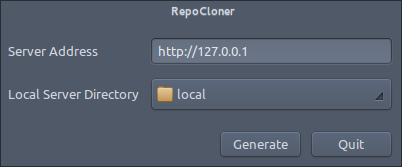
\includegraphics[scale=0.89] {29.png}
  \caption[Screenshot - Repocloner Front End]{Repocloner Front End}
\end{center}
\end{figure}
\begin{figure}[h]
\begin{center}
  % Requires \usepackage{graphicx}
  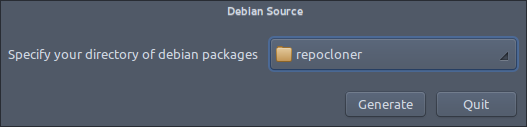
\includegraphics[scale=0.89] {30.png}
  \caption[Screenshot - Repocloner Debian Source Dialog box]{Repocloner Debian Source Dialog box}
\end{center}
\end{figure}\begin{figure}[h]
\begin{center}
  % Requires \usepackage{graphicx}
  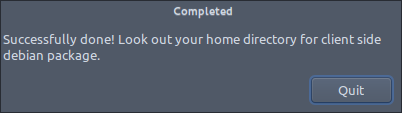
\includegraphics[scale=0.89] {31.png}
  \caption[Screenshot - Repocloner Final Dialog]{Repocloner Final Dialog}
\end{center}
\end{figure}

\chapter{Testing}
\begin{table}[h]
\begin{tabular}{|c|p{5cm}|p{5cm}|p{3cm}|}
  \hline
  Sr. No. & Development & Expected Result & Obtained Expected Results (True/False)\\
  \hline
  1 & Build A basic build. & It shoud boot and work properly. & True\\
  \hline
  2 & Advance build with all essential apps included & It should boot and load properly. & True\\
  \hline
  3 & DMLinux final build with custom GUI & It should render properly. & True\\
  \hline
  4	& OpenGujarat build with translated component & It should show proper translation with proper running. & True\\
  \hline
  5 & MDConverter Application  & It should convert documents as per given specification & True\\
  \hline
  6 & Auto ON Utility Application & It should boot PC as per given time. & True\\
  \hline
  7 & Gujarati Dicitonary & It should display proper meaning. & True\\
  \hline
  \end{tabular}
  \end{table}
  \newpage
  \begin{table}[h]
  \begin{tabular}{|c|p{5cm}|p{5cm}|p{3cm}|}
  \hline
  Sr. No. & Development & Expected Result & Obtained Expected Results (True/False)\\
  \hline
  8 & Debian packages for translations and Gujarati dictionary & It can be installed on other systems & True\\
  \hline
  9 & LAMP front end  & It must do task properly as per given instructions & True\\
  \hline
\end{tabular}
\caption[Test cases]{Test Cases}
\end{table}

\chapter{Future Enhancement}
DMLinux and OpenGujarat both are GNU/Linux Operating systems. Each operating system is build with unique perpose because there is no alternative available.
For future enhancement, there is lots of chances are available for the next years or for the developers also.
For future enhancement purpose, We have made a public repository for all our developed applicaions or operating systems.
\indent Following List of links are public repository for our developments.
\begin{itemize}
\item	DMLinux OS (https://github.com/codejar-lab/dmlinux)
\item	OpenGujarat OS (https://github.com/codejar-lab/opengujarat)
\item	Gujarati Dictionary (https://github.com/codejar-lab/oguj-dict-pkg)
\item	Translation Package(https://github.com/codejar-lab/oguj-trans-pkg) 
\item	Website Source Code(https://github.com/codejar-lab/codejar-lab.github.com)
\item	Auto ON Utility (https://github.com/arpan-chavda/autoon-util)
\item	LAMP Front end (https://github.com/arpan-chavda/lamp-fe-linux)
\item	Multidoc Converter (https://github.com/arpan-chavda/multidocconverter)
\item	Repocloner (https://github.com/arpan-chavda/repocloner)

\end{itemize}


\chapter{Appendix}
\section{Technology Used}
\subsection{Ubuntu Minimal}
\subsubsection{Introduction}
Ubuntu Minimal is an precompiled version of linux kernel with some basic utilities provided with least minimal system.It is just have size of 27 MB.
Current version information:
\begin{itemize}
\item 12.04.1: Long Term Support
\item 12.10: Normal Release
\end{itemize}
We have taken 12.04.1 version as base of OpenGujarat and 12.10 version for DMLinux.
\subsubsection{Free and Open Source}
Ubuntu is well known free and open source gnu/linux operating system. Our both operating systems will be free and open source.
\subsubsection{Open Development}
By making public repository of our both operating system, We are inviting other developers to enhance or fork our operating systems.It is an open development for the people, by the people.
\section{Tools Used}

\subsection{Build essential package}
Build essential pakage contains following dependencies.
\begin{itemize}
\item dpkg-dev (>= 1.13.5)\\
package building tools for Debian
\item g++ (>= 4:4.1.1)\\
The GNU C++ compiler
\item gcc (>= 4:4.1.1)\\
The GNU C compiler
\item libc6-dev \\
GNU C Library: Development Libraries and Header Files\\
or libc-dev
virtual package provided by libc6-dev
\item make\\
The GNU version of the "make" utility.
\end{itemize}

\subsection{chroot environment}

This is the system that will eventually run from the disk. It does not need a kernel, nor a boot-loader unless you are planning on installing it back onto a hard disk (using Ubiquity). The Casper package needs to be installed into the chroot. Casper is what allows the Live System to perform hardware autoconfiguration and run from a live environment. Installing the Casper package will update the kernel�s initrd to perform these tasks. The kernel that is installed into the chroot will be copied out from the chroot and put into the disk image.


\subsection{UCK}
UCK stands for Ubuntu customization toolkit. It is a toolkit to customize any ubuntu based distribution.

\subsubsection{Zenity and YAD framework}
Zenity is GUI framework which uses Glib for backend to create GUI with shell scripts and YAD is fork of zenity and YAD(YAD stands for Yet Another Dialog)provides more features then Zenity.

\begin{itemize}
\item Zenity Version : 3.6.0
\item YAD Version : 0.19.1
\end{itemize}




\chapter{Summary and Conclusion}

\section{Summary}
Summary of activities carried out during major project training at BISAG can be listed as below:
\begin{itemize}
\item Initial Learning about the technologies and the tools.
\item Requirement Analysis of the project.
\item Project Design including GUI related  design.
\item Project Development (Coding).
\item Testing  of the project.
\item Quality Related Work
\item Final  Documentation.
\end{itemize}

\section{Conclusion}
In both distribution various functionalities are implemented.It includes various components that will help users to everday's task in easy wasy. Other utilities development has been developed to enhance user's facilities in the distribution.
As we have developed many things,there are many chances to upgrade those things in future by other developers.

\flushbottom \flushbottom

%\section*{Note for References}
%You may cite reference to any book\cite{HK} or any conference
%\cite{VEC} or any other journal or publication.
%------------------------------------------------------------------------

\newpage

% ------------ Bibliography---------------
%\begin{singlespace}
%\bibliographystyle{plain}
\addcontentsline{toc}{chapter}{\bibname}
%\bibliography{main}
%\end{singlespace}

\begin{thebibliography}{9}
\bibitem{1}
 www.GeoTools.org
\bibitem{2}
  www.sourceforge.net/projects/geotools
\bibitem{3}
  en.wikipedia.org/wiki/GeoTools
\bibitem{4}
  en.wikipedia.org/wiki/GIS
\end{thebibliography}

\end{document}
